% options:
% thesis=B bachelor's thesis
% thesis=M master's thesis
% czech thesis in Czech language
% english thesis in English language
% hidelinks remove colour boxes around hyperlinks

\documentclass[thesis=M,english]{FITthesis}[2012/10/20]

\usepackage[utf8]{inputenc} % LaTeX source encoded as UTF-8

\usepackage{graphicx} %graphics files inclusion
% \usepackage{subfig} %subfigures
% \usepackage{amsmath} %advanced maths
% \usepackage{amssymb} %additional math symbols

\usepackage{listings}
\usepackage{dirtree} %directory tree visualisation
\usepackage{tablefootnote}
\usepackage{subcaption}
\usepackage{eurosym}
\usepackage{amsmath} % to center math equations
\usepackage{pifont}% http://ctan.org/pkg/pifont
\usepackage{enumitem}

\usepackage{minted} % code style
\usepackage{wrapfig} % wrapped images
\usepackage{csquotes} % middle quotes

\newcommand{\HRule}{\rule{\linewidth}{0.5mm}}
\newcommand{\cmark}{\ding{51}}%
\newcommand{\xmark}{\ding{55}}%

%C++
\newcommand{\cpp}{C\nolinebreak\hspace{-.05em}\raisebox{.4ex}{\tiny +}\nolinebreak\hspace{-.10em}\raisebox{.4ex}{\tiny +}}

% Forbid hyphenation
\hyphenation{WhatsApp}

% list of acronyms
% \usepackage[acronym,nonumberlist,toc,numberedsection=autolabel,nomain]{glossaries}
%\iflanguage{czech}{\renewcommand*{\acronymname}{Seznam pou{\v z}it{\' y}ch zkratek}}{}
% \makeglossaries

\newcommand{\tg}{\mathop{\mathrm{tg}}} %cesky tangens
\newcommand{\cotg}{\mathop{\mathrm{cotg}}} %cesky cotangens

\graphicspath{ {images/} }
\lstset{
  basicstyle=\ttfamily,
  columns=flexible,
  breaklines=true,                       % sets automatic line breaking
  breakatwhitespace=true
}

% % % % % % % % % % % % % % % % % % % % % % % % % % % % % % % % % % % 
% % % % % % % % % % % % % % % % % % % % % % % % % % % % % % % % % % % 
\department{Department of Computer Systems}
\title{Security Analysis of the Telegram IM}
\authorGN{Tom{\' a}{\v s}} %author's given name/names
\authorFN{Su{\v s}{\' a}nka} %author's surname
\author{Tom{\' a}{\v s} Su{\v s}{\' a}nka} %author's name without academic degrees
\authorWithDegrees{Bc. Tom{\' a}{\v s} Su{\v s}{\' a}nka} %author's name with academic degrees
\supervisor{Ing. Josef Kokeš}
\acknowledgements{Most importantly, I would like to thank my thesis supervisor Ing. Josef Kokeš for his essential help, guidance and an incredible response time. Many thanks to Jakob Bjerre Jakobsen from the Aarhus University for sharing his source codes of the MTProto illustrations which I partially modified. Thanks to Prof.~Dr.-Ing.~Christof Paar and Dr.-Ing.~Juraj Somorovsky from the Ruhr-University Bochum for encouraging me to pursue this topic. Special thanks to Miriam for proofreading\footnote{In case, she actually does, kind of a test. (TODO)} and last but not least, thanks to my family for supporting me during my studies.}
\abstractCS{TODO}
\abstractEN{TODO}
\placeForDeclarationOfAuthenticity{Žižkov, Prague} %where you have signed the declaration
\keywordsCS{instant messaging, Telegram, MTProto, bezpečná komunikace, bezpečnostní analýza}
\keywordsEN{instant messaging, Telegram, MTProto, secure communication, security analysis}
\declarationOfAuthenticityOption{4} %select as appropriate, according to the desired license TODO

\begin{document}

\begin{introduction}

Instant messaging is a form of an online real-time communication. The history of Instant Messengers (IM) dates back as far as to 1960s, but the modern IMs, as we currently know them, were published in the mid-1990s, such as the very popular ICQ or AOL Instant Messenger. Nowadays, the human interaction and communication take place more and more often in the digital realm and instant messaging is the digital version of a spoken dialogue.

A common feature of the IM software is the ability to see if a specific contact is connected and available or not. Further, IMs are primarily designed for a repetitive exchange of a number of shorter messages, as opposed to the well-established typically longer emails.

Today, many social networks as well provide some form of messaging solution and the users are demanding. Instant messengers are de facto required to have both mobile and web access and more advance capabilities, such as media, voice, or location sharing. Furthermore, the surveillance disclosures emanating from the ex-NSA employee Edward Snowden showed as well the demand for a secure and privacy-aware communication.

In the scope of this thesis we aim to provide a brief overview of the current Instant Messenger solutions with a focus on their security. We will cover the messengers' history, origin, their security-related aspects and other
information in order to provide the reader an insight into the security of
today's modern instant messaging applications.

Following this summary we will focus in more depth on Telegram which stresses out the need for users' privacy, and has 100 million active users, especially popular in Iran, but as well in the US, Germany, India, Uzbekistan, Russia, Italy or Brazil~\cite{telegram-countries}. Telegram introduces its own cryptographic protocol MTProto instead of using known solutions which many of the cryptographic community criticised~\cite{telegram-community-vice,telegram-community-register}. We will devote ourselves to its further investigation, studying the cryptography behind the protocol, how the protocol deals with a key negotiation, message authentication, integrity and other topics.

Furthermore, we will dive into the code of Telegram itself, the official application for Android in particular. We will verify its consistency with the official documentation, focus on its code base, evaluate how it proceeds with user's data storage, and finally in case some inconsistencies are found, we will draft an attack scenario and attempt to execute it.

\end{introduction}


\chapter{Current security status of major IMs}\label{compar}

This chapter contains thorough description of five selected Instant Messengers and its security related findings. Particular software versions are mostly an estimate based on a date some findings were published and the software changelog.

\section{Selection}

We selected the following five Instant Messenger applications. The selection was based on various criterions to create a diverse mixture of messengers. The criterions among others were user base, geographical origin, authors, proclaimed security, license and price. However, we did not want to simply sort the IMs by one of those criterions. We wanted to present an indeed diverse collection. That's why we omitted Facebook Messenger and Apple's iMessage since the first is owned by the very same company as WhatsApp~\cite{facebookwhatsappbuy} and the later is yet another US-based company.

For ease of comparison we decided to select messengers with support for mobile platforms. Particular software versions are mostly an estimate based on a date some findings were published and the software changelog.


\subsection{WhatsApp\protect\footnote{https://www.whatsapp.com}}

Large user base and overall popularity of the application is one of the main reasons WhatsApp is included. With 1 billion active users it is the most used messenger at the moment~\cite{whatsappusers}.

\subsection{Signal\protect\footnote{https://www.whispersystems.org}}

Signal was endorsed by the community in several occasions and is by many considered as the most secure messenger. It's the only messenger completely open-sourced in this collection.

\subsection{Threema\protect\footnote{https://www.threema.ch}}

Threema is the only paid application in this selection. Furthermore Threema comes from Switzerland, and may be therefore considered as an European alternative to the traditionally US-based services.

\subsection{WeChat\protect\footnote{https://www.wechat.com/en/}}

WeChat is with its 700 million active users the most used messenger in China~\cite{wechat-users}. As with Threema we include WeChat mainly for its distinct origin.

\subsection{Telegram\protect\footnote{https://www.telegram.org}}

Telegram praises itself as safer than WhatsApp. It uses its own messaging protocol MTProto and argues for its security. Telegram's clients are open-source but the server side is proprietary. The authors of Russian social network VK, Nikolaj Durov and Pavel Durov, are the creators of Telegram.


\begin{table}[htb]\centering
	\caption{Messengers}
	\label{tab:clients}
	\begin{tabular}{|l|l|l|l|l|}
		\hline
		 \textbf{Name} & \textbf{First release} & \textbf{License} & \textbf{User base} \\ \hline
		WhatsApp & January 2010 & Proprietary & 1 billion\tablefootnote{\label{foot-sep2015}As of February 2016.} \\ \hline
		 Telegram & August 2013 & GPLv2/GPLv3/Proprietary & 100 million\tablefootnote{As of February 2016} \\ \hline
		 Signal & July 2014 & GPLv3 & 10 million\tablefootnote{Signal's predecessor TextSecure as of December 2013.} \\ \hline
		 Threema & 	December 2012  & Proprietary & 3.5 million  \tablefootnote{As of June 2015.} \\ \hline
		 WeChat & January 2011 & Proprietary & 700 million\tablefootnote{As of April 2016.} \\ \hline
	\end{tabular}
\end{table}


\section{Security aspects}

The Electronic Frontier Foundation maintains a scoreboard of messaging applications' security. The scoreboard was initially released in November 2014, and last update occurred on 5 June 2016.

It evaluates messengers based on these seven criteria~\cite{eff-score}:

\begin{itemize}
	\item \textbf{Are messages encrypted in transit?} All user communication is required to be encrypted. Encryption of metadata, such as phone numbers, usernames or dates, is not required. % commas ok
	\item \textbf{Are messages encrypted so the provider can not access it?} All user messages need to be end-to-end encrypted, from the moment user sends a message to the moment the other party receives it. No decrypting  and re-encrypting may occur during that process. The private keys need to be generated at the endpoints, not on a centralized server. Any bulk data collection is therefore meaningless, and no third-party may access the messages unless one party allows it.
	\item \textbf{Can user verify contacts' identity?} This requires a verification mechanism of the other side's identity to prevent Man-in-the-Middle attacks. 
	\item \textbf{Are past communications secure if keys stolen?} All messages need to be encrypted with routinely changed keys. The forward secrecy minimizes consequences when a private key is stolen because the key has only a short-time validity. This criterion requires end-to-end encryption, it is therefore directly dependent on the second criterion.
	\item \textbf{Is the code open to independent review?} Sufficient amount of source-code needs to be available to perform an independent code review. This protects from unintentional encryption flaws, backdoors or bugs.
	\item \textbf{Is the cryptography design properly documented?} The cryptography behind the application needs to be described in detailed documentation.
	\item \textbf{Has there been any recent code audit?} An independent security review of the application is not older than 12 months. This does not require the audit to be publicly available.
\end{itemize}

At the end of each chapter dedicated to one messenger a small note about the received score will be made.

\section{WhatsApp}\label{whatsapp}

WhatsApp is a mobile messaging application. Besides text it enables users to send pictures, videos, voice and locations. WhatsApp Messenger is available for iPhone, BlackBerry, Windows Phone, Android and Symbian~\cite{whatsapphomepage}.

In February 2016 WhatsApp has reached 1 billion active users monthly and was the most used messenger to that moment~\cite{whatsappusers}. The large user base and overall popularity of the application is one of the main reasons WhatsApp is included in this comparison.

Following section describes WhatsApp's security-related incidents.

\subsection{Security-related Incidents}

\subsubsection{Flaws in Registration Process}\label{whatsapp-registration}

WhatsApp's user identity is bound to user's phone number. In order to verify the relationship user has to enter his phone number during the first start-up. WhatsApp server then sends SMS with verification code to this number. User submits the code from the received text message and WhatsApp creates his account.  

\begin{figure}[htb]
	\centering
	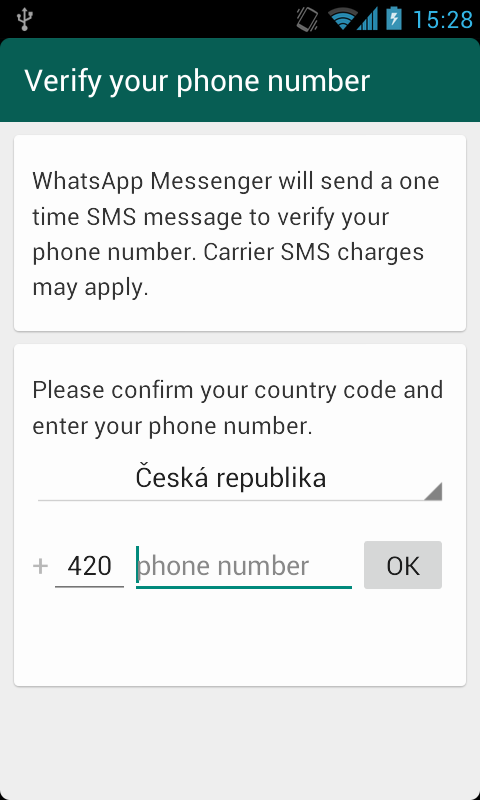
\includegraphics[width=0.4\textwidth]{whatsapp-registration.png}
	\caption[WhatsApp's registration process]{WhatsApp's registration process prompts the user to enter his phone number, and verifies it by sending a text message.}
	\label{img:whatsapp_reg}
\end{figure}

Up to version 2.6.5, WhatsApp offered an alternative verification process. Instead of the user waiting for a text message, he was rather supposed to send a SMS to one of WhatsApp's phone numbers where he included his email. WhatsApp later sent verification code to the email and user verified himself with this code~\cite{whatsapp-shootingthemsg}.

Serious drawbacks were found in this method in 2011~\cite{whatsapp-hijack1}. To hijack user's account attacker first opted for this method. Then using SMS spoofing service he sent SMS to WhatsApp's phone number pretending it originates from the victim. Attacker set the content of the message to an email he owned leading to WhatsApp sending the verification code to the attacker. The attacker then simply entered the code from an email and successfully hijacked the victim's account.

Following these findings another method to bypass the registration process was published. During the registration phase WhatsApp sent a request for the verification SMS to be sent to the client in HTTP request similiar to this~\cite{whatsapp-shootingthemsg}:

\begin{listing}[htb]
\caption{HTTP request to dispatch a text message to the client for verification.}
\begin{minted}{http}
GET [..]?to=4915143[..]&auth=659&[..] HTTP/1.1
User-Agent: WhatsApp/2.6.4 iPhone_OS/4.3.3 Device/iPhone_4
\end{minted}
\label{lst:status-whatsapp-http}
\end{listing}

The request contained the final verification code in the GET parameter. This led to a conclusion the client created the verification code, not the server, and expected user's confirmation. An attacker could simply intercept the request, retrieve the verification code and make sure the request did not arrive to WhatsApp's servers to make the victim unaware of the malicious intentions.

The attacker created a fake HTTP OK response to let the messenger think the request was successful, and then entered the retrieved verification code from the intercepted request. The attacker successfully hijacked the victim's WhatsApp identity and could both send and receive all the victim's messages.

The author of the attack scenario notified WhatsApp developers beforehand and WhatsApp fixed the issue before the research was made public~\cite{whatsapp-shootingthemsg}. To the date of writing this thesis, WhatsApp does not offer the discussed verification method anymore.


\subsubsection{Password generation}

WhatsApp uses slightly modified version of the XMPP protocol~\cite{whatsapp-xmpp}. During the registration process it creates a username based on the user's phone number. In newer versions than 2.10 the password is generated on server's side~\cite{whatsapp-imei}. However, older versions used the phone's IMEI  number as password~\cite{whatsapp-imei, whatsapp-imei2}.

\begin{listing}[htb]
\caption{Pseudo-code of the password generation on Android in older versions of WhatsApp.}
\begin{minted}{c}
md5(revert(<IMEI>))
\end{minted}
\label{lst:status-whatsapp-password}
\end{listing}


Any phone number and IMEI was therefore all an attacker needed to send messages on victim's behalf. Numerous applications are collecting plenty of user data, and the IMEI and phone number might be among them. Any database leak with such information would lead directly to large accounts abuse.

\subsubsection{Messages encryption}

Up to version 2.8 approximately, WhatsApp did not use any message encryption. The messenger used port 443 (commonly used for HTTPS) to send content, however it did not encrypt anything whatsoever~\cite{whatsapp-plaintext}. Using a simple network sniffer like Wireshark an attacker was able to read all user's messages.

On May 2012, an application called WhatsAppSniffer was released~\cite{whatsapp-sniffer, whatsapp-sniffer2}. It abused the previously described flaw and enabled the attacker to see all the victim's messages in easy and lucid user interface.

\begin{figure}[htb]
	\centering
	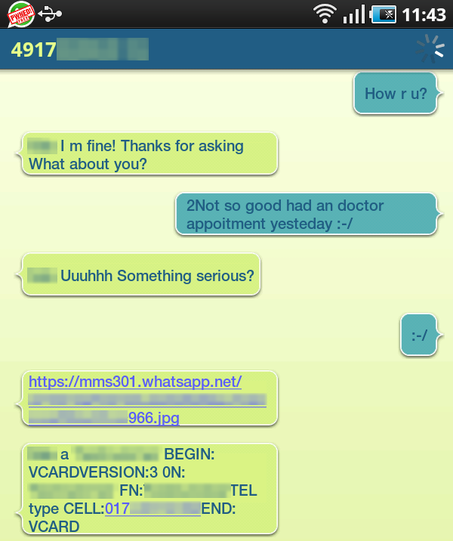
\includegraphics[width=0.4\textwidth]{whatsapp-sniffer.png}
	\caption[WhatsAppSniffer]{WhatsAppSniffer application was able to sniff all the user's data and read them~\cite{whatsapp-sniffer2}.}
	\label{img:whatsapp_sniffer}
\end{figure}


In August 2012, WhatsApp started to use some sort of encryption. The developers did not reveal which protocol they used or any other information. Reports showed that simple message sniffing, as described in the previous paragraph, seized to work~\cite{whatsapp-sniffernomore}. Some sources claim the  RC4 stream cipher was used for encryption~\cite{whatsapp-rc4,whatsapp-rc42}.

On November 18, 2014, Open Whisper Systems, the creators behind Signal messenger, announced a partnership with WhatsApp. The partnership should have escalated into incorporating OWS' encryption protocol to WhatsApp bringing end-to-end encryption to all WhatsApp clients. Open Whisper Systems stated: \emph{``we are moving quickly towards a world where all WhatsApp users will get end-to-end encryption by default''}~\cite{openwhisperwhatsapp}. At that time WhatsApp confirmed the partnership, however did not comment it any further nor offered any further information. WhatsApp's FAQ only briefly stated that \emph{``WhatsApp communication between your phone and our server is encrypted''}~\cite{whatsapp-faq}.

In April 2015, \emph{heise.de} investigated the current state of WhatsApp's encryption. The journalists were sniffing messages using the Man-in-the-Middle technique. They showed that Android versions used end-to-end encryption and that the messages were encrypted according to the TextSecure protocol~\cite{whatsapp-encstate}. However, during an analysis of the iOS client they concluded the messages weren't protected in such manner. Finally, they concluded they are unsure whether end-to-end encryption was actually used in all cases.

In April 2016, WhatsApp finally released an official white paper confirming all its messages are end-to-end encrypted with the use of Signal Protocol. The document thoroughly described all aspects and encryption methods. It stated \emph{``WhatsApp messages, voice and video calls between a sender and receiver that use WhatsApp client software released after March 31, 2016 are end-to-end encrypted.''} \cite{whatsapp-whitepaper}.


\subsection{EFF's secure messaging score}

At the time of writing, WhatsApp has six points out of seven in the EFF's secure messaging scorecard~\cite{eff-score}.

\begin{table}[htb]
	\centering
	\caption{WhatsApp's secure messaging score}
	\label{my-label}
	\begin{tabular}{|l|l|}
		\hline
		Are messages encrypted in transit? & \cmark \\\hline
		Are messages encrypted so the provider can not access it? & \cmark \\ \hline
		Can user verify contacts' identities? & \cmark \\ \hline
		Are past communications secure if keys stolen? & \cmark \\ \hline
		Is the code open to independent review? & \xmark \\ \hline
		Is the cryptography design properly documented? & \cmark \\ \hline
		Has there been any recent code audit? & \cmark \\ \hline
	\end{tabular}
\end{table}


\section{Signal}

Signal is an open-source voice calling and messaging application. It is available for Android and iOS. Its messages are end-to-end encrypted. During a voice call a simple identity check is available when a given word is supposed to be pronounced by both sides of the call.

Signal uses its own Signal Protocol (previously called Axolotl) based on cryptographic primitives such as Elliptic Curves (Curve25519), AES and HMAC-SHA256~\cite{signal-bochum}. As mentioned in Section~\ref{whatsapp} WhatsApp currently uses the very same protocol.

\subsection{Security-related incidents}

In late 2014 \emph{Der Spiegel} published articles claiming NSA considered Signal's encrypted voice calling used with other tools as a catastrophic to theirs surveilance missions~\cite{signal-spiegel}. Edward Snowden recommended Signal on various occasions~\cite{signal-snowden,signal-snowden2}.

A research team from the Ruhr-University Bochum provided a security analysis \emph{``How Secure is TextSecure?''} of the former Signal version \cite{signal-bochum}. They came to a conclusion that the protocol is susceptible to an Unknown key-share attack and proposed a mitigation. The researchers concluded Signal as secure in case the suggested patch was applied which eventually was.

Up to this date no other security-related incidents or analysis of Signal messenger are known.

\subsection{EFF's secure messaging score}

Signal fulfilled all the requirments in the EFF's secure messaging scorecard and received a full score~\cite{eff-score}.

\begin{table}[htb]
	\centering
	\caption{Signal's secure messaging score}
	\label{my-label}
	\begin{tabular}{|l|l|}
		\hline
		Are messages encrypted in transit? & \cmark \\\hline
		Are messages encrypted so the provider can not access it? & \cmark \\ \hline
		Can user verify contacts' identities? & \cmark \\ \hline
		Are past communications secure if keys stolen? & \cmark \\ \hline
		Is the code open to independent review? & \cmark \\ \hline
		Is the cryptography design properly documented? & \cmark \\ \hline
		Has there been any recent code audit? & \cmark \\ \hline
	\end{tabular}
\end{table}


\section{Threema}

Threema is a paid IM application available for all three major platforms -- Android, iOS and Windows Phone. Text messaging, multimedia, locations, voice messages and file sharing are supported. Threema is developed in Switzerland and all servers are located in the very same place.

Threema is a paid application. As of December 2016 the price was set to \euro2.99. Threema is using user IDs and linking user's phone number and email address is not required.

\subsection{Security-related incidents}

In August 2015, Threema was auditted by an external company. The Threema documentation states~\cite{threema-audit}: \emph{``The result confirms that Threema's concepts fully meet the requirements for secure and trustworthy instant messaging.''} The full audit is available on Threema's web page.

The main point of Threema's criticism is considered with its closed-source nature therefore the inability to verify its source code. There are no other security analysis.

\subsection{EFF's secure messaging score}

In the EFF's comparison Threema missed a single point for not completing an indenpendent code review~\cite{eff-score}.

\begin{table}[htb]
	\centering
	\caption{Threema's secure messaging score}
	\label{my-label}
	\begin{tabular}{|l|l|}
		\hline
		Are messages encrypted in transit? & \cmark \\\hline
		Are messages encrypted so the provider can not access it? & \cmark \\ \hline
		Can user verify contacts' identities? & \cmark \\ \hline
		Are past communications secure if keys stolen? & \cmark \\ \hline
		Is the code open to independent review? & \xmark \\ \hline
		Is the cryptography design properly documented? & \cmark \\ \hline
		Has there been any recent code audit? & \cmark \\ \hline
	\end{tabular}
\end{table}


\section{WeChat}

WeChat is a Chinese mobile messenger available to all major mobile platforms including iOS, Android, Windows Phone and BlackBerry. Besides regular text messages, WeChat offers media, location, video sharing and even games. As of May 2016, WeChat had 700 million active users~\cite{wechat-users}.

A special business versions of WeChat was introduced in April 2016 named Enterprise WeChat focused on companies communication offering few additional features.

\subsection{Censorship}

The Internet censorship in China blocks extensive amount of web sites including web giants such as Facebook, Twitter or Google~\cite{china-twitter,china-facebook}.

Since WeChat's servers are located in China, it is subjected to such restrictions. Users are required to agree and obey specific rules, such as \emph{``upholding the socialist system, social morality and authenticity of information''}~\cite{china-imblocking}. The Chinese government reasons for such actions to allegedly build a cleaner cyberspace and to ensure the national security~\cite{china-blocking2}.

\subsection{Security-related incidents}

WeChat operators are capable of accessing messages, contacts and even user's location. Numerous states including United States, India and China itself expressed concerns over WeChat being a threat to their national security issues~\cite{wechat-states}.

\subsubsection{XcodeGhost malware}

In 2015, Apple reported WeChat was infected with XcodeGhost malware~\cite{wechat-xcodemalware}. The malware was able to obtain user device information, read clipboard, prompt alert dialog and other. Apple claimed the malware was not able to perform any significant damage, and could not access any user data.

\subsection{EFF's secure messaging score}

Regrettably, WeChat was not included in the EFF secure messaging survey.


\section{Telegram}

Telegram is an instant messaging service enabling users to send messages, photos, videos, stickers and files. Telegram describes itself as fast and secure solution for instant messaging, and claims to be safer than WhatsApp. Compared to WhatsApp, Telegram is more cloud-based because it stores all messages on its servers, and sync them with all the user's devices~\cite{telegramfaq}.

Nikolaj and Pavel Durov are the authors of Telegram. After leaving the social network VK Pavel Durov founded they focused on creating safe forms of communication leading to Telegram.

Telegram provides two modes of messaging. Apart from the regular chat, Telegram provides so-called \emph{secret chats}. Secret chat messages are end-to-end encrypted and are not stored on the Telegram's servers for longer period of time than necessary~\cite{telegramfaq}.

\begin{figure}[htb]
	\centering
	\label{A}
	\begin{subfigure}[b]{0.4\textwidth}
		\centering
		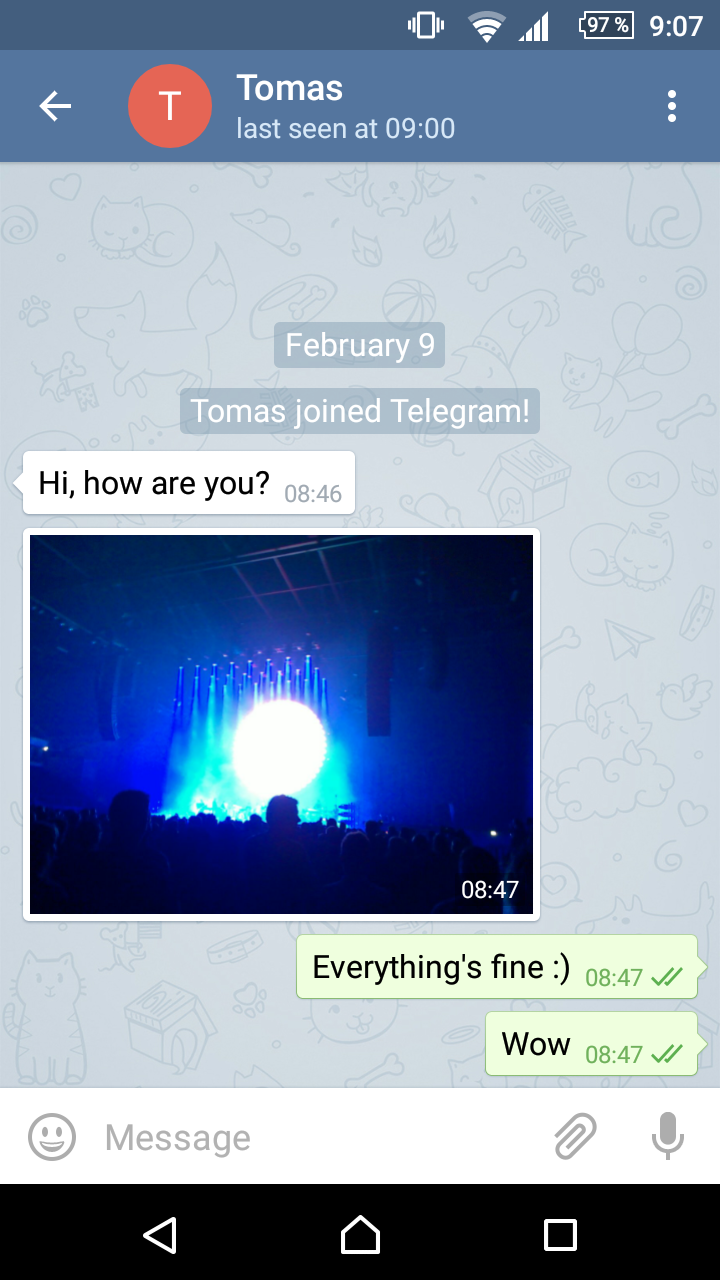
\includegraphics[width=0.9\textwidth]{telegram-regular.png}
		\caption{Regular chat}
		\label{img:telegram:regular}
	\end{subfigure}
	\hfill
	\begin{subfigure}[b]{0.4\textwidth}
		\centering
		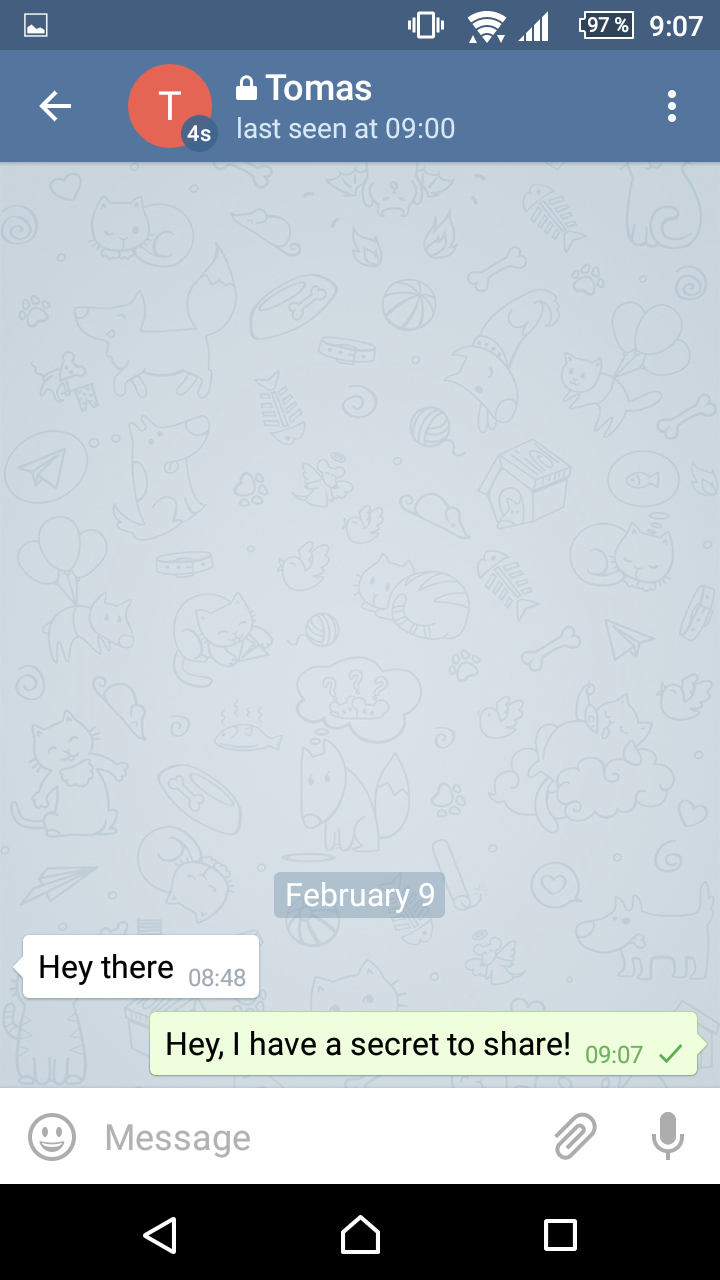
\includegraphics[width=0.9\textwidth]{telegram-secret.png}
		\caption{Secret chat}
		\label{img:telegram:secret}
	\end{subfigure}
	\caption[Telegram chat modes]{Telegram has two chat modes. Regular chat is meant to be used for traditional communication, and its messages are stored on Telegram's servers. Secret chats are supposed to provide another layer of protection, and are end-to-end encrypted.}
\end{figure}

Similar to WhatsApp user can contact someone using his phone number, but Telegram provides classical username focused approach as well. User needs to know the recipient's phone number or Telegram username in order to communicate with him.

All clients are licensed under GPLv2 or GPLv3 license, the server-side part of Telegram is closed-sourced and proprietery~\cite{telegram-server}.

In 2015, Brazilian judiciary ordered WhatsApp to shut down its service for 48 hours. During this event, which was finally lowered to only 12 hours, Telegram welcomed 5 million new users \cite{whatsappbrazil}. It may be therefore considered as a direct competitor to WhatsApp.

In May 2015 Telegram had 62 million active users~\cite{telegram-users}.


\subsection{Security-related incidents}

\subsubsection{SMS authentication}

In Section~\ref{whatsapp-registration} we described how the WhatsApp's registration process using SMS works. Telegram works on a similar basis, and allows as well logging in using just a simple SMS.

The text messages are fully readable for mobile network operators which may and usually do cooperate with the corresponding government. Furthermore, SMS can be intercepted using inexpensive IMSI catchers. If an attacker is able to steal the authenticating SMS, he is able to login on his behalf. Worse, Telegram stores the whole user's message history, thus it allows the attacker to read older messages as well.

In early 2016, it was shown this is a legitimate concern~\cite{telegram-smsiran}. Some Telegram users experienced their accounts being erased, and blamed Telegram to enforce political censorship which Telegram denied. Russian activist Oleg Kozlovsky described in its Facebook post~\cite{telegram-russia} how his account was allegedly hacked.

First the Russia's mobile operator disabled SMS service on Oleg's phone number. Upon the disconnection, the attacker tried to log into the victim's Telegram account. Because intercepting the SMS is all the attacker needs, he simply entered the authorization code he sniffed, and got full access to Oleg's account. Telegram recommended to turn on two-factor authentication for additional security.

These concerns raise serious questions if SMS authentication is a security-wise valid instrument.

\subsubsection{Cracking Contest}

On November 4, 2014, Telegram published contest with a winning price \$300,000 for cracking its encryption. The contest became quite known in the community, and probably provided a bit of advertisement for Telegram.

The contest remained unsolved until its closure. Number of authors considered it rigged, and stated that the contest does not provide any prove of Telegram's overall security whatsoever~\cite{telegramcontestfail,telegramcontestfail2}.

\subsubsection{IND-CCA insecurity}

In Spring 2015, researchers from Aarhus University performed an independent audit of the protocol~\cite{telegram-aarhus}. They concluded the encryption scheme is not IND-CCA\footnote{Indistinguishability under Chosen Ciphertext} secure, meaning any ciphertext can be altered into another ciphertext decrypting to the very same plaintext.

The researchers stressed the theoretical nature of the attack and that they \emph{``do not see any way of turning the attack into a full plaintext-recovery attack''}~\cite{telegram-aarhus}. Telegram's FAQ describes it as a minor issue unaffecting overall security~\cite{telegram-techfaq}.


\subsection{EFF's secure messaging score}

As mentioned Telegram has two types of messages. Telegram is therefore evaluated twice by the EFF.


\subsubsection{Telegram regular chats}

\begin{table}[htb]
	\centering
	\caption{Telegram regular chat's secure messaging score}
	\label{tab:telegram-regular-eff}
	\begin{tabular}{|l|l|}
		\hline
		Are messages encrypted in transit? & \cmark \\\hline
		Are messages encrypted so the provider can not access it? & \xmark \\ \hline
		Can user verify contacts' identities? & \xmark \\ \hline
		Are past communications secure if keys stolen? & \xmark \\ \hline
		Is the code open to independent review? & \xmark \\ \hline
		Is the cryptography design properly documented? & \cmark \\ \hline
		Has there been any recent code audit? & \cmark \\ \hline
	\end{tabular}
\end{table}


\subsubsection{Telegram secret chats}

\begin{table}[htb]
	\centering
	\caption{Telegram secret chat's secure messaging score}
	\label{tab:telegram-secret-eff}
	\begin{tabular}{|l|l|}
		\hline
		Are messages encrypted in transit? & \cmark \\\hline
		Are messages encrypted so the provider can not access it? & \cmark \\ \hline
		Can user verify contacts' identities? & \cmark \\ \hline
		Are past communications secure if keys stolen? & \cmark \\ \hline
		Is the code open to independent review? & \cmark \\ \hline
		Is the cryptography design properly documented? & \cmark \\ \hline
		Has there been any recent code audit? & \cmark \\ \hline
	\end{tabular}
\end{table}







\chapter{Cryptography behind Telegram}\label{telegramcrypto}

Telegram authors decided to craft a brand new encryption scheme supposedly to achieve better delivery times and stability, MTProto. In this section we describe into details how the protocol should work based on~\cite{telegram-aarhus} and the official Telegram documentation.


\section{Initialization}\label{crypto-initialization}

During the first launch of Telegram application user needs to enter and verify its telephone number. The verification is done by sending a five digit code to the phone via SMS. The user then enters the code into the app and therefore verifies its phone number. When this process is done the registration process begins as follows.

Suppose a client $C$ is registering to server $S$:

\begin{enumerate}
	\item $C$ sends a 128-bit random integer \emph{nonce} to $S$.
	\item $S$ responds with another 128-bit random integer \emph{server\_nonce}, composite number \emph{pq} and a fingerprint of a RSA public key.
	\item $C$ provides a proof of work by decomposing \emph{pq} into prime factors \emph{p} and \emph{q} such that $\emph{p} < \emph{q}$.
	\item $C$ has several RSA public keys stored locally and chooses the appropriate one based on the received fingerprint.
	\item $C$ crafts a payload of \emph{p}, \emph{q}, \emph{pq}, \emph{nonce}, \emph{server\_nonce} and another new 256-bit random integer \emph{new\_nonce}. The payload including its hash is then encrypted by the RSA key and sent to $S$.
	\item $S$ responds with $g$, $g_a$ and $p$ encrypted AES-IGE using a key derived from \emph{new\_nonce} and \emph{server\_nonce}.\label{crypto-initialization-6}
	\item $C$ generates random 2048-bit $b$ and computes $g_b = g^b \bmod p$ and $K = g_a^b \bmod p$. The $g_b$ value is sent to $S$ encrypted in the way as previously.
	\item $S$ calculates $K = g_b^a \bmod p$. Both $C$ and $S$ now share a common key $K$ noted as \texttt{auth\_key}.
\end{enumerate}

Some details may be omitted for simplification. During the exchange the client should check following requirements:\label{crypto-prime-req}

\begin{itemize}
	\item $p$ is a safe prime, meaning $q = \frac{p-1}{2}$ needs to be prime as well
	\item $2^{2047} < p < 2^{2048}$
	\item $g$ is equal to 2, 3, 4, 5, 6 or 7 and it generates a cyclic subgroup of prime order $q$
	\item $1 < g_a, g_b < p-1$
	\item and is recommended to check $2^{2048-64} < g_a, g_b < p - 2^{2048-64}$
\end{itemize}

The requirements check might be cached and the client is as well allowed to hard-code the already checked $p$ and $q$ values into the application.

We compared these requirements with the FIPS 186-4 publication concerning Digital Signature Algorithm and concluded it requires similar conditions as Telegram with only minor distinctions.

The resulting \texttt{auth\_key} is now used for all client-server communication and regular chats. Finally, a fingerprint of the exchanged \texttt{auth\_key} is created labeled as \texttt{auth\_key\_id}. It is crafted from the last 64 bits of SHA-1(\texttt{auth\_key}).



\section{Regular chats}\label{crypto-regular}

With the connection to server established in the previous section, we may now look into the delivery process. The~\cite{telegram-aarhus} was concerned with secret chats only, therefore in this section we relay on the official documentation only.


\subsection{Payload}\label{crypto-regular-payload}

First, let's describe the content of a single message, further referred to as a payload. The payload prior to encryption is depicted in Figure \ref{img:regular-payload} and contains:

\begin{figure}[htb]
	\centering
	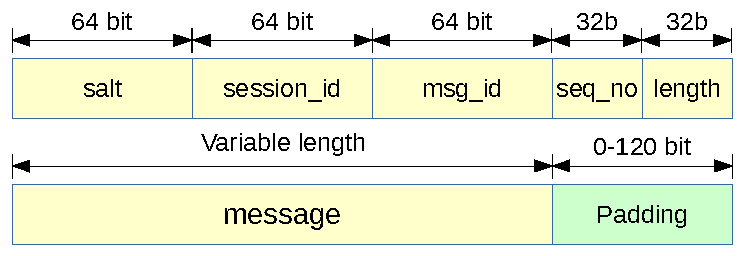
\includegraphics[width=0.7\textwidth]{regular-payload.pdf}
	\caption[Message payload in regular chats]{Payload of a single message to be encrypted in regular chat contains salt, session and message identifier, sequence number, length and the text itself.}
	\label{img:regular-payload}
\end{figure}

\begin{itemize}
	\item \textbf{salt} Periodically changed number used for replay attacks protection and other.
	\item \textbf{session\_id} Unique number to identify the user and its device.
	\item \textbf{msg\_id} Unique ID of the message within a session.
	\item \textbf{seq\_no} Message sequence counter.
	\item \textbf{length} Length of the actual message.
	\item \textbf{message} Text of the actual message.
\end{itemize}


\subsection{Encryption}\label{crypto-regular-enc}

The whole encryption process is visualized in Figure \ref{img:crypto-regular-enc}.

First, the message key \texttt{msg\_key} is calculated. It is composed of the first 128 least significant bits of the SHA-1 hash of the payload to be encrypted. Next, the array is padded with 0-120 random bits in order to be divisible by the AES block size -- 128 bits.

This \texttt{msg\_key} along with the \texttt{auth\_key} described in Section \ref{crypto-initialization} are taken as input into the Key Derivation Function (KDF) which performs number of SHA-1 hashes and truncation yielding two 256-bit values: the AES key and the IGE initialization vector (IV) used for encrypting this particular message.

\begin{figure}[htb]
	\centering
	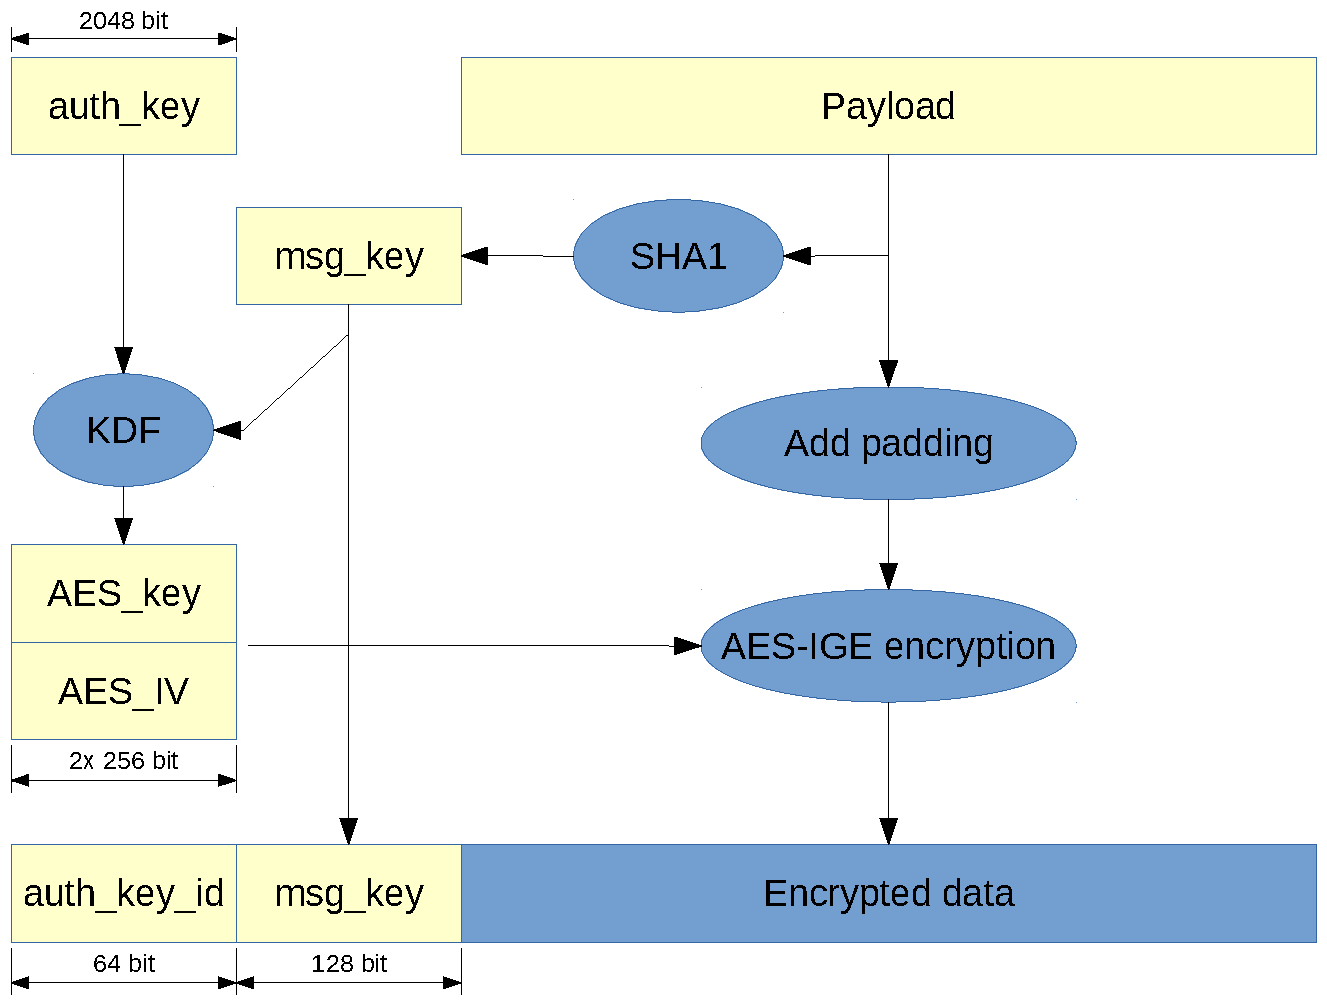
\includegraphics[width=1\textwidth]{mtproto-encflow.pdf}
	\caption[MTProto encryption flow]{The AES key and IV is derived from the \texttt{auth\_key} and SHA-1 hash of the payload \texttt{msg\_key}. Using these values the padded payload is encrypted. The encrypted data along with \texttt{auth\_key\_id} and \texttt{msg\_key} are ready to be transported~\cite{telegram-aarhus}.}
	\label{img:crypto-regular-enc}
\end{figure}

Finally, two other values are added at the top of the encrypted data array: the already mentioned \texttt{msg\_key} and the \texttt{auth\_key\_id} described in Section \ref{crypto-initialization}. This data array is then ready to be transported to the server.

\subsubsection{Advanced Encryption Standard}

The Advanced Encryption Standard (AES) is a symmetric block cipher with key lengths of 128, 192 and 256 bits respectively and block size of 128 bits. Telegram uses 256 bit key. AES is currently the most widely used symmetric cipher and is used in many internet standards such as IPsec, TLS, SSH and many others~\cite{understanding-crypto}.

AES was selected through a worldwide open competition and finally defined in the FIPS-197 publication by the US National Institute of Standards and Technology (NIST) in 2001. As of today, AES is secure against brute-force attacks and no reasonable analytic attacks are currently known~\cite{understanding-crypto}.

\subsubsection{Infinite Garble Extension}

Infinite Garble Extension (IGE) is a lesser-known block cipher mode. It is shown on Figure \ref{img:crypto-regular-ige-enc} and defined by the following formula~\cite{telegram-openssl-ige}:

\begin{gather*}
c_i = f_K(m_i \oplus c_{i-1}) \oplus m_{i-1}
\end{gather*}

where $f_K$ stands for the encrypting function with key $K$ (AES in our case) and $i$ goes from 1 to $n$ -- the number of plaintext blocks.

Careful reader notices that for the first output block we need two initialisation values $m_0$ and $c_0$. Both are taken from the IV values described earlier. The original paper described $m_0$ as a random block and $c_0$ its encrypted counterpart. The OpenSSL implementation however, uses a more general implementation where both $m_0$ and $c_0$ are provided by the user~\cite{telegram-openssl-ige}.

\begin{figure}[htb]
	\centering
	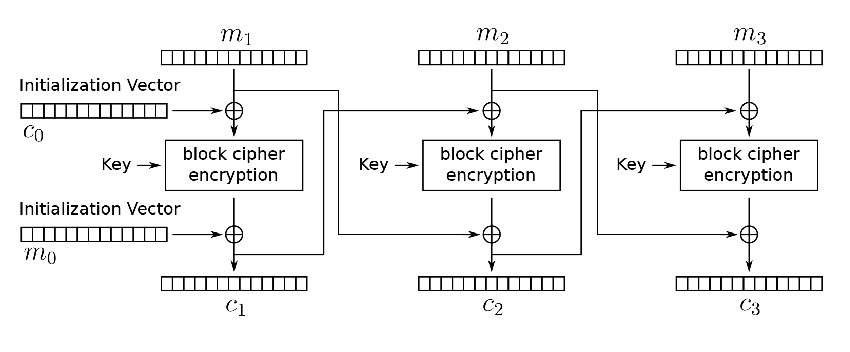
\includegraphics[width=1\textwidth]{ige-enc.pdf}
	\caption[IGE block cipher mode]{IGE mode of operation with two Initialization Vectors used with AES~\cite{telegram-aarhus}.}
	\label{img:crypto-regular-ige-enc}
\end{figure}

\subsubsection{SHA-1}

SHA-1 is a cryptographic hash function and most widely used one~\cite{understanding-crypto}. It produces 160-bit digest of a message. The authors opted for SHA-1 because of its low resource consumption~\cite{telegram-sha1}. Some experts consider SHA-1 as outdated and recommended to be replaced by SHA-2 or SHA-3~\cite{telegram-sha1}. % TODO consequences for Telegram tady nebo jinde?

\subsection{Decryption}\label{crypto-regular-dec}

Before the decryption process starts the \texttt{auth\_key\_id} is validated. The receiver's \texttt{auth\_key\_id} needs to match the value the sender appended to the byte array. If the values differ the whole message is discarded.

\begin{figure}[htb]
	\centering
	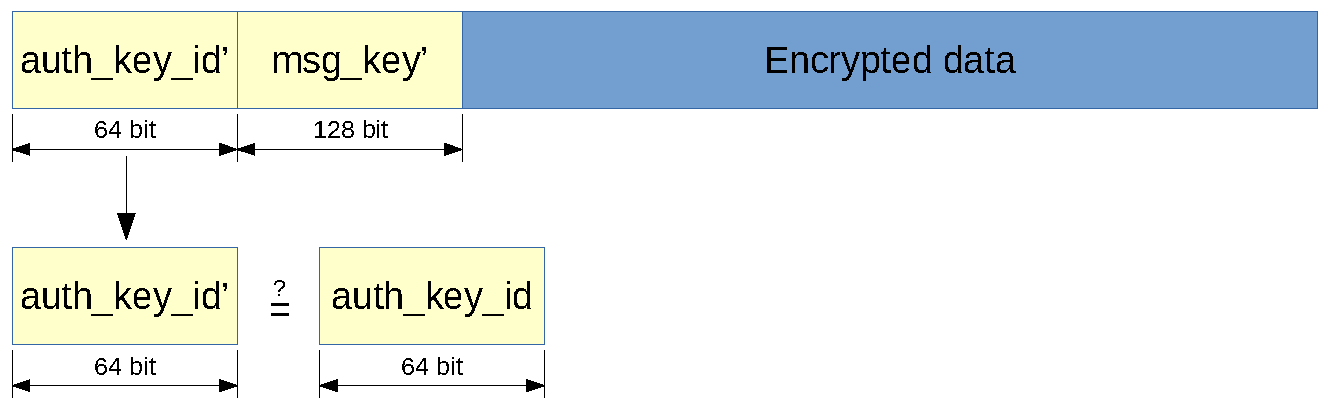
\includegraphics[width=0.9\textwidth]{mtproto-auth-key.pdf}
	\caption[Message acceptance check]{Before the decryption process starts the \texttt{auth\_key\_id} values are checked.}
	\label{img:crypto-regular-dec}
\end{figure}

The decryption process is plainly the encryption process in reverse. The KDF yields the AES key and IV values used for decrypting the data. The padding is stripped and the SHA-1 of the payload generates \texttt{msg\_key} which is compared to \texttt{msg\_key'}. The whole process is lucidly visualized in Figure \ref{img:telegram-decflow}.

\begin{figure}[htb]
	\centering
	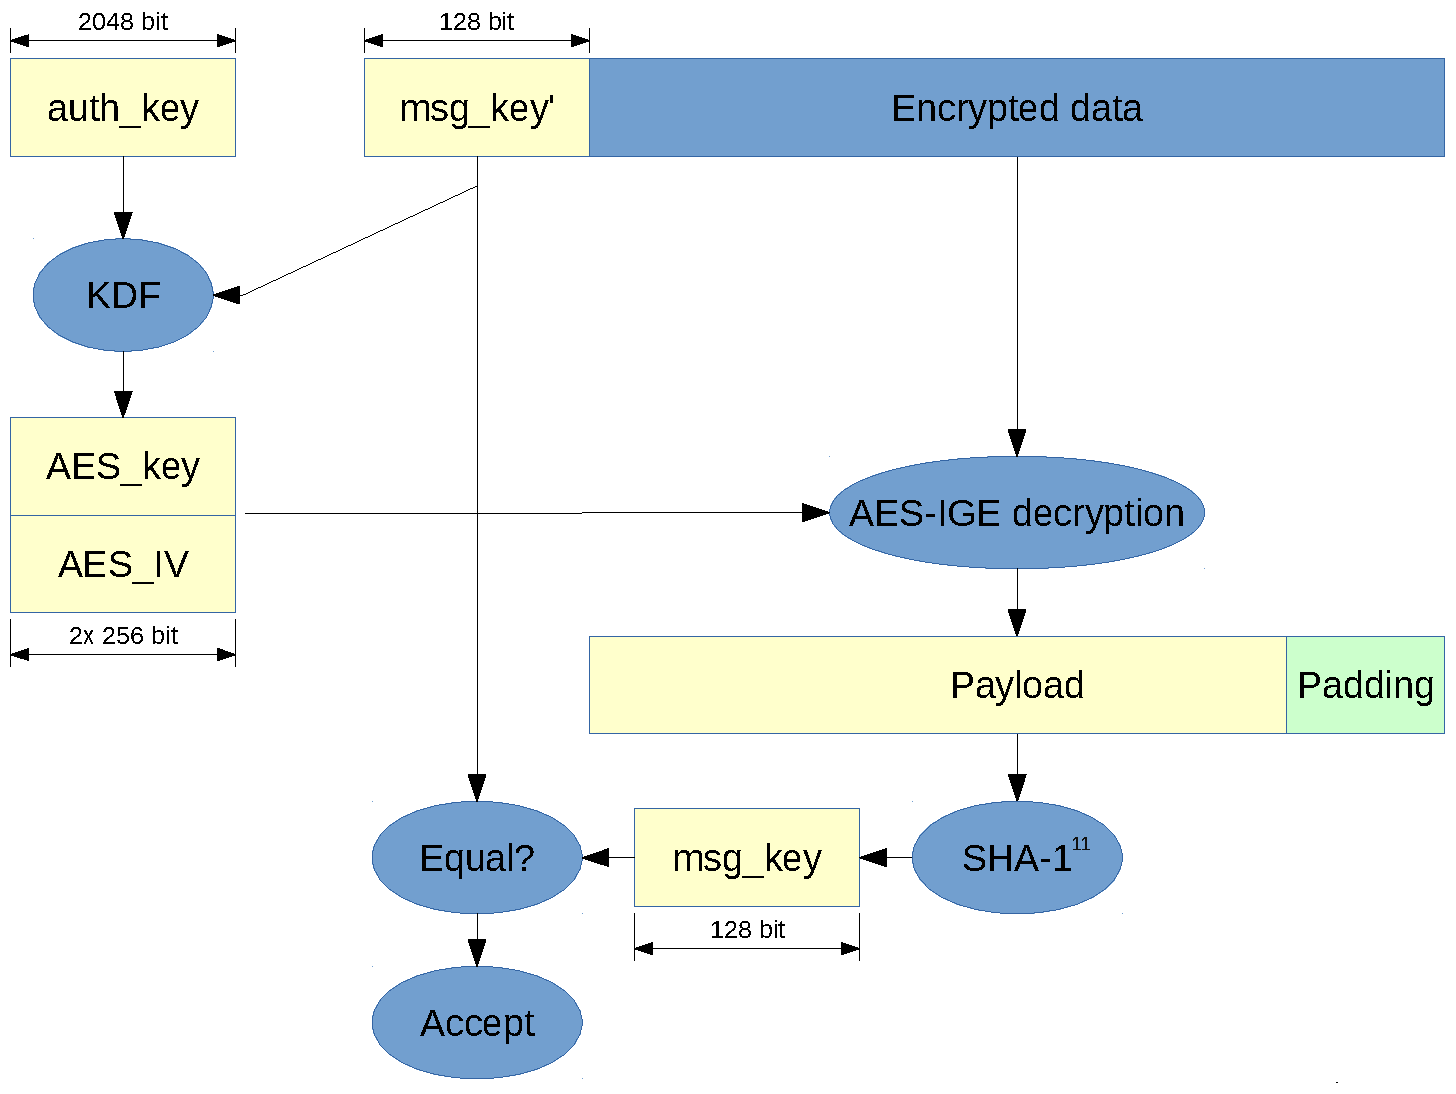
\includegraphics[width=1\textwidth]{mtproto-decflow.pdf}
	\caption[MTProto decryption flow]{The KDF produces the AES key and IV from the \texttt{auth\_key} and received \texttt{msg\_key'}. The SHA-1 of the decrypted payload generates \texttt{msg\_key} which is compared to \texttt{msg\_key'} and only then accepted~\cite{telegram-aarhus}.}
	\label{img:telegram-decflow}
\end{figure}




\section{Secret chats}\label{crypto-secret}

Secret chats are designed to bring an extra level of security compared to regular chats. Secret chat may be initiated between two particular devices only and therefore the messages may be read only on those devices.

It is crucial to note that all secret chat communication is done using the connection described previously in \ref{crypto-initialization}. All data described as follows are considered as input into the MTProto protocol for regular chats. Hence the data are actually encrypted twice.% More on that in TODO

\subsection{Key exchange}\label{crypto-keyexchange}

The exchange performs traditional Diffie-Hellman key exchange (DH). The DH parameters are received from the Telegram server and the client verifies them in the very same manner as in Section \ref{crypto-prime-req}. The exchange proceeds similarly as earlier, however with the connection already established is a little more straightforward. Suppose user $A$ initiates secret chat with $B$:

\begin{enumerate}
	\item $A$ computes a random 2048-bit number $a$ and sets $g_a = g^a \bmod p$.\label{enum:DH-a}
	\item $B$ receives the request on all of its authorized devices and an exclusive one accepts it.
	\item $B$ generates random $b$ and sets $g_b = g^b \bmod p$\label{enum:DH-b}.
	\item Both users calculate the master key $K = g_a^b \bmod p = g_b^a \bmod p$. $K$ is the secret chat's master key denoted \texttt{auth\_key} as well.
\end{enumerate}

Worth mentioning, in secret chats key exchange the client generates its \emph{a} (\emph{b} respectively) in the following way:
\begin{gather*}
a = r_{client} \oplus r_{server}
\end{gather*}

Where $r_{client}$ is a 2048-bit random integer generated on the client side and $r_{server}$ is 2048-bit random integer generated on the server side. These values are then XORed constructing the client's secret value. This is performed to mitigate the client's poor capabilities to generate a cryptographically secure random number as concerned Android in August 2013~\cite{telegram-android-securerandom}.

\begin{figure}[htb]
	\centering
	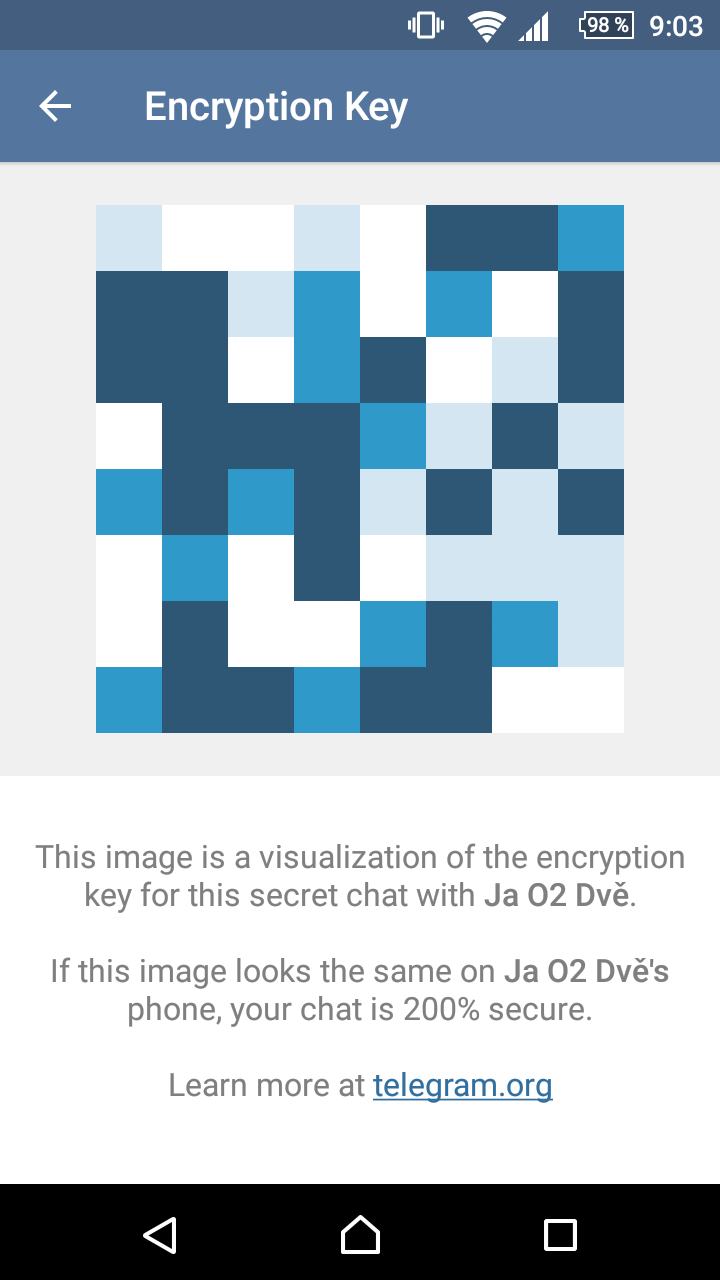
\includegraphics[width=0.4\textwidth]{telegram-keybox.png}
	\caption[Encryption key visualization]{Encryption key visualization provides a technique to verify no malicious intermediary is present.}
	\label{img:telegram-keybox}
\end{figure}

The DH by itself does not provide any authentication of the communicating parties and is therefore susceptible to an active Man-in-the-Middle attack. To mitigate this issue the user is provided with an option to display counterpart's encryption key. Telegram creates a white-blue box to visualize the key as may be seen on Figure~\ref{img:telegram-keybox}. To make sure no malicious mediator is present users are supposed to meet in person and verify the keys are identical. There is no such mechanism in regular chats.

The visualisation used to be based on a 128-bit fingerprint\footnote{Not to be confused with the 64-bit \texttt{auth\_key\_id} fingerprint.} of the secret key. An~article presented in January 2015 showed~\cite{telegram-264} that when the attacker forces (e.g. socially engineers) both sides to initiate the secret chat, a MiM attack is possible only with $2^{64}$ operations, rather than $2^{128}$, based on the Birthday paradox. The article claims the attack is possible for a well financed adversary and estimates the attack to cost tens of millions USD. Telegram's FAQ addresses this issue and states its cost is around a trillion dollars to achieve a result in one month. Nevertheless, Telegram later decided to use additional 160 bits from the key summing up to 288 bits~\cite{telegram-techfaq}. This improvement should make this attack impossible.

The article as well reasons that in real-world scenario the users don't actually meet to verify the key. Most of them probably ignore the verification whatsoever, some send the image via regular chat or using another -- possibly insecure -- channel.

To accomplish the Perfect Forward Secrecy model the key is renegotiated each time it has been used for more than 100 messages or has been used for more than one week. For the renegotiation the already established chat is used in order to send the $g_a$ and $g_b$ values. The server does not help with the randomness here and the same DH parameters are used. The \emph{auth\_key} visualization does not change and is therefore based on the first negotiated key.

It is unclear whether Telegram applies the Trust on first mechanism.


\subsection{Payload}

With the key negotiated we may now focus on the message encryption itself. Let's describe the payload which slightly differs from its regular chat counterpart. It is composed of:

\begin{figure}[htb]
	\centering
	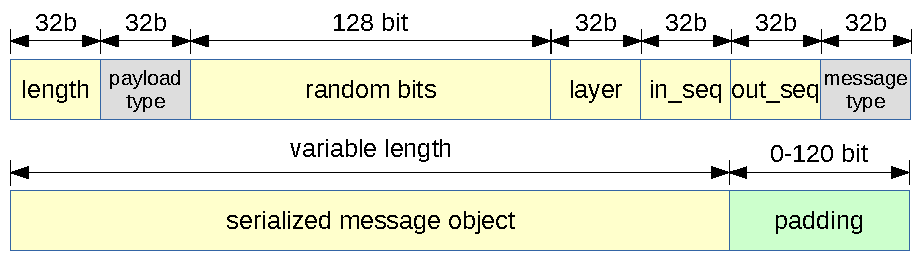
\includegraphics[width=0.95\textwidth]{secret-payload.pdf}
	\caption[Message payload in secret chats]{Payload of a single message in secret chat contains a number of additional fields~\cite{telegram-aarhus}.}
	\label{img:crypto-secret-payload}
\end{figure}

\begin{itemize}
	\item  \textbf{length} The length of the payload excluding padding and the length itself.
	\item  \textbf{payload type} Header related to the protocol version and the message type.
	\item  \textbf{random bits} 120 random bits generated by the author followed by 8 bits to specify the length of it in bytes.
	\item  \textbf{layer} Integer specifying the protocol version.
	\item  \textbf{in\_seq} Message counter for incoming messages.
	\item  \textbf{out\_seq} Message counter for outgoing messages.
	\item  \textbf{message type} Header related to the protocol version and the message type.
	\item  \textbf{serialized message object} Containing other values and the message itself as depicted in Figure \ref{img:crypto-secret-messageobject}.
\end{itemize}

Both payload and message type are not described into much details in the documentation. \cite{telegram-aarhus} states they're both \emph{''headers related to the version of the protocol``}. The serialized message object contains four subsequent values:

\begin{figure}[htb]
	\centering
	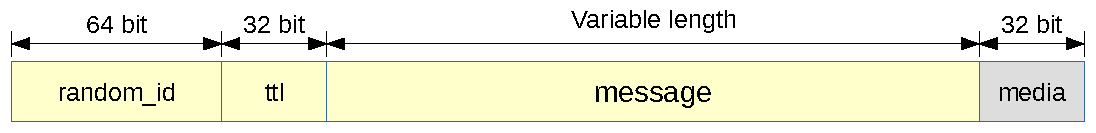
\includegraphics[width=1\textwidth]{decrypted-message.pdf}
	\caption[Message object]{The message object contains the message itself, random integer, time to live settings and media header.}
	\label{img:crypto-secret-messageobject}
\end{figure}

\begin{itemize}
	\item \textbf{random\_id} Random value assigned by the author to identify the message; also sent as a plaintext.
	\item  \textbf{ttl} Time to live, an integer specifying the lifetime of a message in seconds. This concerns the so-called self-destruct mechanism.
	\item \textbf{message} The actual text of a message provided by the user.
	\item \textbf{media} Header specifying media attachment if any.
\end{itemize}

Throughout this paper we assume that no media attachments are present and therefore the \texttt{media} attribute is always empty. This payload is then serialized as an array of bytes and prepared to be encrypted.

\subsection{Encryption}\label{crypto-secret-enc}

The encryption process is the same as seen in Figure \ref{img:crypto-regular-enc}. As mentioned at the beginning the outcome of the encryption then servers as an input to MTProto regular communication.

\subsection{Decryption}\label{crypto-secret-dec}

Decryption is the same as well. First the \texttt{auth\_key\_id}s are validated.  Then the decryption process starts exactly in the same way as in Figure \ref{img:crypto-regular-dec}.





\chapter{The Analysis}\label{analysis}

In this chapter we present our approach and share some of the findings we discovered. These findings are based primarily on these three sources:

\begin{itemize}
	\item The official open-sourced Telegram application for Android
	\item The official Telegram documentation
	\item The already cited~\cite{telegram-aarhus}
\end{itemize}

We commenced by installing Telegram for Android and analyzing it with various tools in order to perform comparison with the other sources. The following section describes our actions.

\section{Setup}\label{analysis-setup}

First, we cloned the official Telegram repository. Since we realized a simple code exploration is not satisfactory due to both complexity and poor code quality we installed the following software.

To run and potentially debug the application Android SDK is needed. Further, the Android NDK is required as well, since Telegram uses the JNI as mentioned earlier. For a complete developer-like experience the Android Studio was installed. Android Studio is the official IDE for Android platform and is based on the popular IntelliJ IDEA platform~\cite{android-studio}.

A mobile phone running rooted Android operating system was connected to a computer with such software. The Android Studio itself deals with the phone-computer connection (using the \emph{adb} software) and performs building, compiling and transferring the final .apk file to the phone. It as well enables the developer to debug the software which was crucial here for better understanding of the Telegram's code.

Further, we wanted to sniff the data sent from the application. To achieve that two approaches were used.

\subsection{Sniffing using wireless hotspot}

In the first scenario we set up a wireless network on the computer and instruct the mobile to connect to it. Even though this does require the victim to connect to the network, there are ways to achieve this by using special dedicated devices~\cite{pineapple}. The Diagram \ref{img:analysis-setup-hotspot} shows this setup.

\begin{figure}[htb]
	\centering
	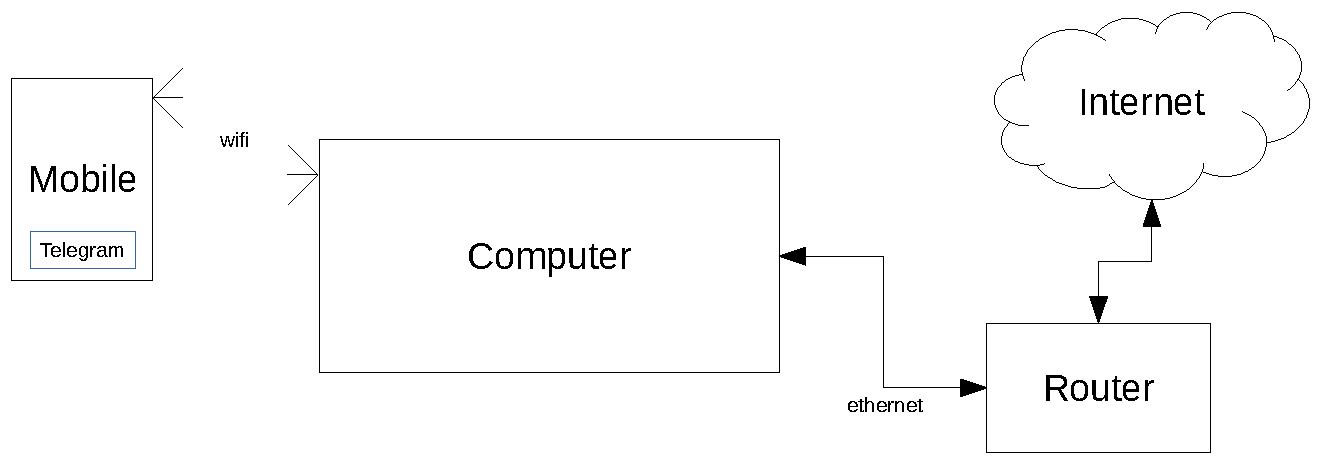
\includegraphics[width=1\textwidth]{setup-hotspot.pdf}
	\caption[Analysis setup 1]{Computer running analysis software is connected to the internet on one interface and creating WiFi hotspot using the other one. Mobile phone running Telegram connects to the computer's WiFi and all data are therefore routed through the computer.}
	\label{img:analysis-setup-hotspot}
\end{figure}

This scenario is easy to setup because most Operating Systems support this functionality out of the box. The only downside is that we need two network interfaces -- one for creating the hotspot and another to connect to the internet.


\subsection{Sniffing using ARP Poisoning}

To demonstrate we may omit the hotspot setup and perform the analysis without forcing the mobile to change its network we're introducing second scenario shown in Figure \ref{img:analysis-setup-arp}. In this case the computer and the mobile phone are in the same network.

\begin{figure}[htb]
	\centering
	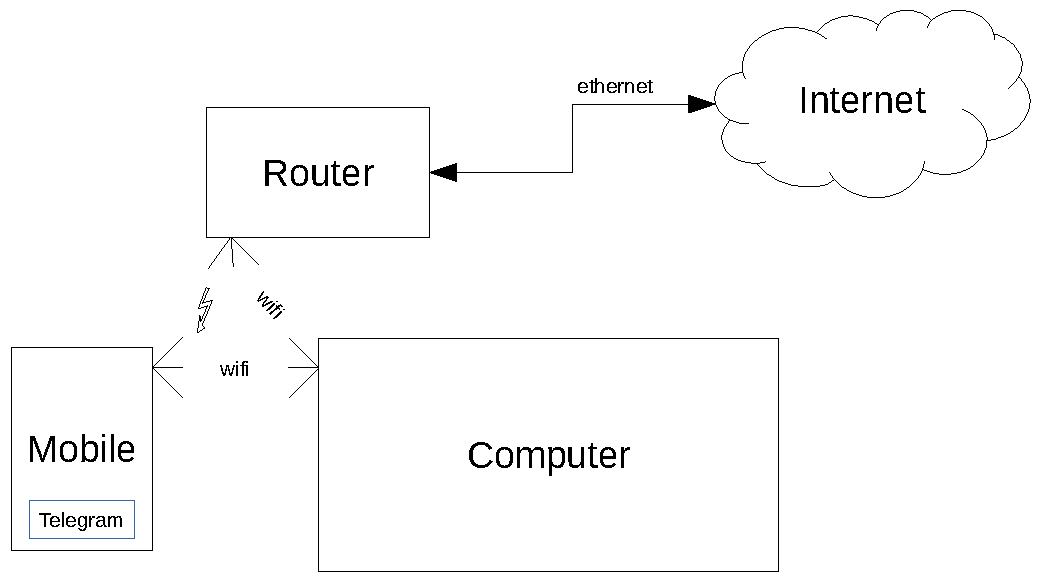
\includegraphics[width=1\textwidth]{setup-arp.pdf}
	\caption[Analysis setup 2]{Both computer and mobile are connected to the same network. Computer runs ARP Poisoning software inducing the mobile to send traffic through the computer.}
	\label{img:analysis-setup-arp}
\end{figure}


By using Ettercap, a \emph{``comprehensive suite for man in the middle attacks''}~\cite{ettercap-homepage} available in Kali Linux, we launched an ARP Poisoning attack against the phone.

Address Resolution Protocol (ARP) is a protocol which transforms an Internet layer address into a link layer address. Typically, this might be the mapping of an IPv4 address to an Ethernet address. ARP Poising, or ARP spoofing, is a technique by which the attacker sends fake ARP packets to the victim claiming his Ethernet address is associated with an IP address different than truly his.

We launched this attack against the phone and the router, meaning the phone sent all communication to the computer instead of directly sending it to the gateway and vice versa. Since all communication is now flowing through the computer we may thoroughly analyze it.

This setup is as well convenient if we are not able to use WiFi as a hotspot, for example due to the need of it for the internet connection itself. Beware that this setup should be used in test networks only.

\section{Code}

The application is publicly available on Github~\cite{github-telegram} with the first commit dating back to late October 2013. This thesis is concerned with the latest Telegram version 3.13.1 as up to date in October 2016, the \texttt{64e8ec3} commit in particular.

The application's main programming language is Java but it uses the Java Native Interface (JNI) to incorporate C libraries such as borringssl, ffmpeg, sqlite and others. Since the 3.2.2 version Telegram moved a significant portion of logic into a separate C library called \emph{tgnet}. The library is responsible for many connection-related actions including communication with the server and sending messages. The codebase closely resembles the previous Java code. The secret messages are still dealt within the Java part of the application.

It should be noted that since this was introduced in the 3.2.2 version (September 2015) whereas the~\cite{telegram-aarhus} analysis is based on 2.7.0 (April 2015) and therefore wasn't concerned with the \emph{tgnet} library whatsoever.

\subsection{Code quality}

We decided to analyze the code quality using static code analysis tools to avoid opinion-based reviews. Android Studio itself comes with a code scanning tool \emph{lint}~\cite{android-studio-lint}. The tool seeks for potential bugs, optimization improvements, security, performance and other.

Lint was run using the default settings and yielded 20 errors and 286 warnings. The full output is attached in the appendix. Android Studio can as well perform code inspections. It runs lint and adds number of checks such as error handling, security, code style, javadoc, spelling etc. It found over 650 000 issues in the Telegram project. The results are as well available in the appendix. % TODO

It is important to note that the code analysis concerns the project as whole meaning it includes all the dependencies. Some issues may therefore relate to the libraries Telegram uses not to Telegram itself.

Further, some files contain upto thousands of lines and multiple classes in one file. For example the \emph{TLRPC.java} has 23,010 lines containing 873 static classes. For a brief comparison we are including Table \ref{tab:analysis-storage-metrics} comparing some of the Telegram metrics with Signal. The comparison excludes all libraries, binaries, assets etc. and discusses the source code related files only. We leave it to the reader to draw her own conclusions.

\begin{table}[htb]\centering
	\caption{Telegram vs Signal code metrics}
	\label{tab:analysis-storage-metrics}
	\begin{tabular}{|l|l|l|}
		\hline
					& \textbf{Telegram} & \textbf{Signal} \\ \hline
		Project size\tablefootnote{The project as a whole, including all libraries, assets etc.} & 188,6 MB & 138,6 MB \\ \hline
		Largest file by size & 714.6 KB\tablefootnote{\path{TMessagesProj/src/main/java/org/telegram/tgnet/TLRPC.java}} & 87.4 KB\tablefootnote{\path{src/org/thoughtcrime/securesms/util/Base64.java}} \\ \hline
		Largest file by lines count & 23,009 &  2,096 \\ \hline
		Number of test files\tablefootnote{Number of files each including at least one unit test.} & 0 & 13 \\ \hline
TODO         &  & \\ \hline
	\end{tabular}
\end{table}

It should be noted Signal's files are well documented which impacts on its size. That is not the case of Telegram at all.

\section{Storage}\label{analysis-storage}

In this section we briefly look how Telegram stores its data. All data are stored in the \path{org.telegram.messenger/files} folder. Two types of files are present, SQLite database file and \path{.dat} files which are in Telegram's own configuration format:

\begin{itemize}
	\item \path{cache4.db} SQLite database file.
	\item \path{tgnet.dat} Main configuration data.
	\item \path{dcXconf.db} Number of Datacenter specific configuration files.
\end{itemize}

The \path{cache4.db} file is a SQLite database file. It contains 38 tables in total containing contacts, messages, chat information and all other user data. Messages are stored in bytes and therefore de facto in plaintext. Since the database is available only by physical access to the phone, we do not see this as a malpractice.

The \path{tgnet.dat} file is a place where Telegram stores its configuration directives. It contains configuration version, currently used datacenter ID, session IDs, time synchronization values, timestamps and other. For each datacenter -- Telegram stored 5 during our analysis -- it stores its ID, IPv4 and IPv6 addresses, salts and most importantly the secret \texttt{auth\_key} and \texttt{auth\_key\_id} fingerprint.

\subsection{Extraction scripts}\label{analysis-storage-scripts}

To proper analyze the data Telegram stores we wrote three scripts, all in Python 3. The scripts address the \path{tgnet.dat} file, regular messages and encrypted chat information both stored in the SQLite database. Examples of those files are included in the \path{examples} folder of the project and a brief readme file describing how to run the scripts is present as well. Some values' meaning is unclear, therefore the scripts print a simple question mark in such cases to indicate this.

\subsubsection{Extracting tgnet.dat}

The \path{tgnet-extractor.py} parses the \path{tgnet.dat} file and prints all the values to standard output. This file has Telegram's own binary format and in a nutshell is a collection of values simply written one by one, with no keys, formatting or structure. The most useful values are the datacenter's IP addresses and the \texttt{auth\_key} secrets, mainly \texttt{auth\_key\_id} we expected to see in the sniffed traffic, more on that in the following Section \ref{analysis-obf}.

\subsubsection{Extracting messages}

Next script \path{message-extractor.py} works with the bytes stored in the SQLite database, the column \emph{data} in table \emph{messages} in particular. Those bytes store information on one single message sent in a regular chat.

The script extracts values such as message ID, values to identify both the sender and the receiver, timestamps, flags and most importantly the UTF-8 encoded string of the message itself.

\subsubsection{Extracting secret chat information}

Last but not least the \path{encrypted-chat-extractor.py} script is responsible for the bytes in the column \emph{data} of \emph{enc\_chats} table. Among others it describes a secret chat instance and contains ID, dates, identification values and yet again an \texttt{auth\_key} secret. Note that this \texttt{auth\_key} is used for this particular secret chat which is then encrypted with the regular chat \texttt{auth\_key} as described in Section \ref{crypto-secret}.

\section{Undocumented obfuscation}\label{analysis-obf}

During the data collection the received data did not correspond with the documentation. We expected the data to be in a form of \texttt{auth\_key\_id}, \texttt{msg\_key} and encrypted data; see Figure \ref{img:analysis-obf-expected}.

\begin{figure}[htb]
	\centering
	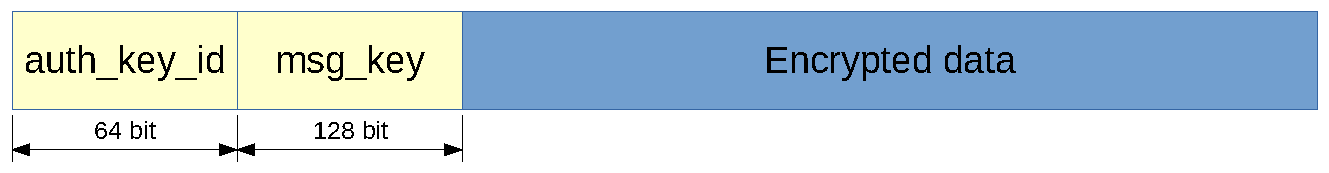
\includegraphics[width=1\textwidth]{sniffed-expected.pdf}
	\caption[Expected form of sniffed data]{Expected form of sniffed data where 64-bits of key fingerprint are followed by \texttt{msg\_key} and encrypted data.}
	\label{img:analysis-obf-expected}
\end{figure}

Using the scripts described in \ref{analysis-storage-scripts} we extracted our testing \texttt{auth\_key} and \texttt{auth\_key\_id} from our device in order to compare it with the sniffed data. \texttt{auth\_key\_id} was not present. The whole packet seemed random and therefore likely encrypted.

We examined the code and discovered the responsible function for this behavior is the \texttt{Connection::sendData} function located in \path{TMessagesProj/jni/tgnet/Connection.cpp} file. Before sending the data in the expected manner, they are encrypted one more time with a random key attached in front of the data. Interestingly the Counter block mode is used instead of the IGE endorsed by Telegram.

To properly explain the obfuscation method we are introducing our own terminology first to add a little more clarity because Telegram doesn't practise a great job naming variables.

\subsection{Terminology}

Since the variables are explained into more details in the following sections, reader may skip this list and use it as a reference later on. The titles we are introducing are:

\begin{itemize}
	\item \textbf{obf\_enc\_key\_bytes} 64 random bytes storing \textbf{obf\_enc\_key} and \textbf{obf\_enc\_iv} used for obfuscation. Telegram calls this plainly \emph{bytes}.
	\item \textbf{obf\_enc\_key} The key used for encryption to obfuscate data.
	\item \textbf{obf\_enc\_iv} The IV used for encryption to obfuscate data.
	\item \textbf{obf\_dec\_key\_bytes} 64 bytes derived from \textbf{obf\_enc\_key\_bytes} storing the server's encryption key and IV. Labeled in Telegram as \emph{temp}.
\end{itemize}

\subsubsection{Temporary encryption key}\label{code-obf-enc-key}

The process starts by generating 64 random bytes \texttt{obf\_enc\_key\_bytes}. The first 8 bytes are unused. The bytes 8 -- 40 are used as an encryption key and bytes 41 -- 56 as an IV. Bytes 57 -- 64 are composed of the last 8 bytes of \texttt{obf\_enc\_key\_bytes} encryption of itself. It is unclear what are those bytes used for. The final \texttt{obf\_enc\_key\_bytes} to be sent is visualized in Figure \ref{img:code-obfuscation-bytes-sent}.

\begin{figure}[htb]
	\centering
	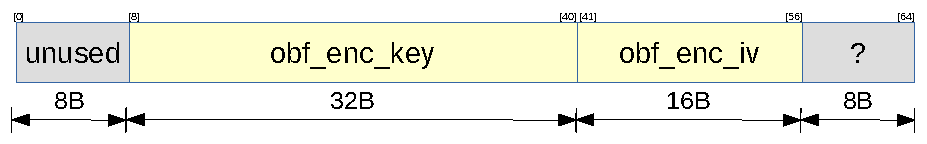
\includegraphics[width=1\textwidth]{bytes-sent.pdf}
	\caption[Random bytes used for obfuscation]{The \texttt{obf\_enc\_key\_bytes} containing random bytes and its usage for the obfuscation encryption.}
	\label{img:code-obfuscation-bytes-sent}
\end{figure}

Further, the length of the packet, yet again encrypted and the real data to be transmitted as expected from the official documentation are then AES-CTR encrypted using the \texttt{obf\_enc\_key} and \texttt{obf\_enc\_iv} and sent. All other data in this TCP stream are encrypted using the same obfuscation key. When another connection is established a new \texttt{obf\_enc\_key\_bytes} is generated and the process repeats.

\subsubsection{Temporary decryption key}

Besides the \texttt{obf\_enc\_key\_bytes} setup the very same function deals with setting up the \texttt{obf\_dec\_key\_bytes}. This temporary key is used for decrypting incoming traffic.

The \texttt{obf\_dec\_key\_bytes} is derived from the \texttt{obf\_enc\_key\_bytes}. Totally 48 bytes are reversed from \texttt{obf\_enc\_key\_bytes} starting at position 8. This may be seen in Listing \ref{lst:code-obf-dec}. The first 32 bytes are then set as a decryption key for incoming traffic and next 16 bytes for IV.

\begin{listing}[htb]
\caption{Temporary decryption key deduction from the \texttt{obf\_enc\_key\_bytes} array. First 32 bytes are used as a decryption key, next 16 bytes for the IV.
\protect \\ Telegram for Android source code, file \texttt{Connections.cpp}, line 331.}
\label{lst:code-obf-dec}
\begin{minted}{C++}
for (int a = 0; a < 48; a++) {
    obf_dec_key_bytes[a] = obf_enc_key_bytes[55 - a];
}
\end{minted}
\end{listing}


We believe Telegram server receives the \texttt{obf\_enc\_key\_bytes}, tampers them in a way described in this section and finally encrypts its response with \texttt{obf\_dec\_key\_bytes}. As mentioned earlier, this is officially not documented whatsoever. Yet again, a more conventional approach would be much appreciated such as the usage of SSL/TLS, a cryptographic protocol scrutinized thoroughly by researchers all over the world.

To sum up, the whole function is depicted in Listing \ref{lst:analysis-obfuscation} in its simplified version. It as well uses our own terminology to concur with this section.

\begin{listing}[htb]
\caption{The function starts by generating random bytes. The decryption key is then derived and both encrypt and decrypt keys are set. Finally, the length of the payload (as well obfuscated), the \texttt{obf\_enc\_key\_bytes} and the actual IGE encrypted payload are sent. The function's argument -- the payload -- is in the expected form as depicted in Figure \ref{img:analysis-obf-expected}.
\protect\linebreak Telegram for Android source code, file \texttt{Connection.cpp}, line 289, redacted.}
\label{lst:analysis-obfuscation}
\begin{minted}{C++}

void sendData(payload)
{
    obf_enc_key_bytes = byte[64];

    if (!firstPacketSent) {
        obf_dec_key_bytes = byte[64];
        fillWithRandom(obf_enc_key_bytes);

        for (int a = 0; a < 48; a++) {
            obf_dec_key_bytes[a] = obf_enc_key_bytes[55 - a];
        }

        setAESEncryptKey(obf_enc_key_bytes + 8);
        setEncryptIv(obf_enc_key_bytes + 40);

        setAESDecryptKey(obf_dec_key_bytes);
        setDecryptIv(obf_dec_key_bytes + 32);
        
        send(obf_enc_key_bytes);
        firstPacketSent = true;
    }

    send(AESCTREncrypt(packetLength));
    send(AESCTREncrypt(payload))
}
\end{minted}
\end{listing}

\subsection{Deobfuscation program}\label{analysis-obf-program}

To verify these findings and to continue the analysis we created software to deobfuscate the traffic. Even though the first language of choice was Python to contain all the scripts in one package, we finally opted for \cpp. This has two major advantages, one we can be directly inspired by the Telegram code, and second we can access OpenSSL functions directly the same way Telegram does.

The program is capable of fetching the obfuscation key and transforming the data into its deobfuscated form and further analyze. It takes two or three arguments as an input:

\begin{itemize}

	\item \textbf{incoming stream} sniffed incoming data
	\item \textbf{outgoing stream} sniffed outgoing data
	\item \textbf{key} file containing the user's \texttt{auth\_key} (optional)

\end{itemize}

The first and second arguments are binary files of the sniffed traffic. Since the \texttt{obf\_enc\_key\_bytes} are sent by the client it is stored in the outgoing stream and it is therefore not possible to deobfuscate any traffic without this data. We used Wireshark repeatedly to follow the TCP stream and then saving both incoming and outgoing data into a binary file. This proved as a viable technique.

The third argument is optional. It is the user's secret \texttt{auth\_key}. This is obviously not available for an attacker, but it is helpful for studying purposes. When extracted user may see the real traffic Telegram generates and what actions are taken.

Readme file is present describing how to build and run the program.



\section{Replay attack}\label{analysis-attacks}

During the analysis we as well examined some parts of the code attempting to discover some potential vulnerabilities to exploit. To provide a little bit of a context let's now briefly describe how Telegram processes any incoming data.

\subsection{Incoming data processing}

The Figure \ref{img:analysis-replay-incoming} shows how Telegram processes all incoming data. First, the \texttt{Connection::onReceivedData()} function is called and incoming data are deobfuscated in the way described in Section \ref{analysis-obf}.

Next, the \texttt{ConnectionsManager::onConnectionDataReceived()} function is called. If the \texttt{auth\_key\_id} is not set to 0 (which is only the case of the key exchange process; see Section \ref{crypto-keyexchange}) the \texttt{Datacenter::decryptServerResponse()} is invoked. This function checks the \texttt{auth\_key\_id} and if valid decrypts the actual payload using the master secret \texttt{auth\_key} and derived \texttt{msg\_key}. Upon doing so the message ID and other checks are performed.

If the decryption succeeds the \texttt{onConnectionDataReceived()} function proceeds and processes further the IGE decrypted payload. It checks all the headers and other fields. Finally, if all checks succeed the whole process is finalized by the \texttt{ConnectionsManager::processServerResponse} function.

\begin{figure}[htb]
	\centering
	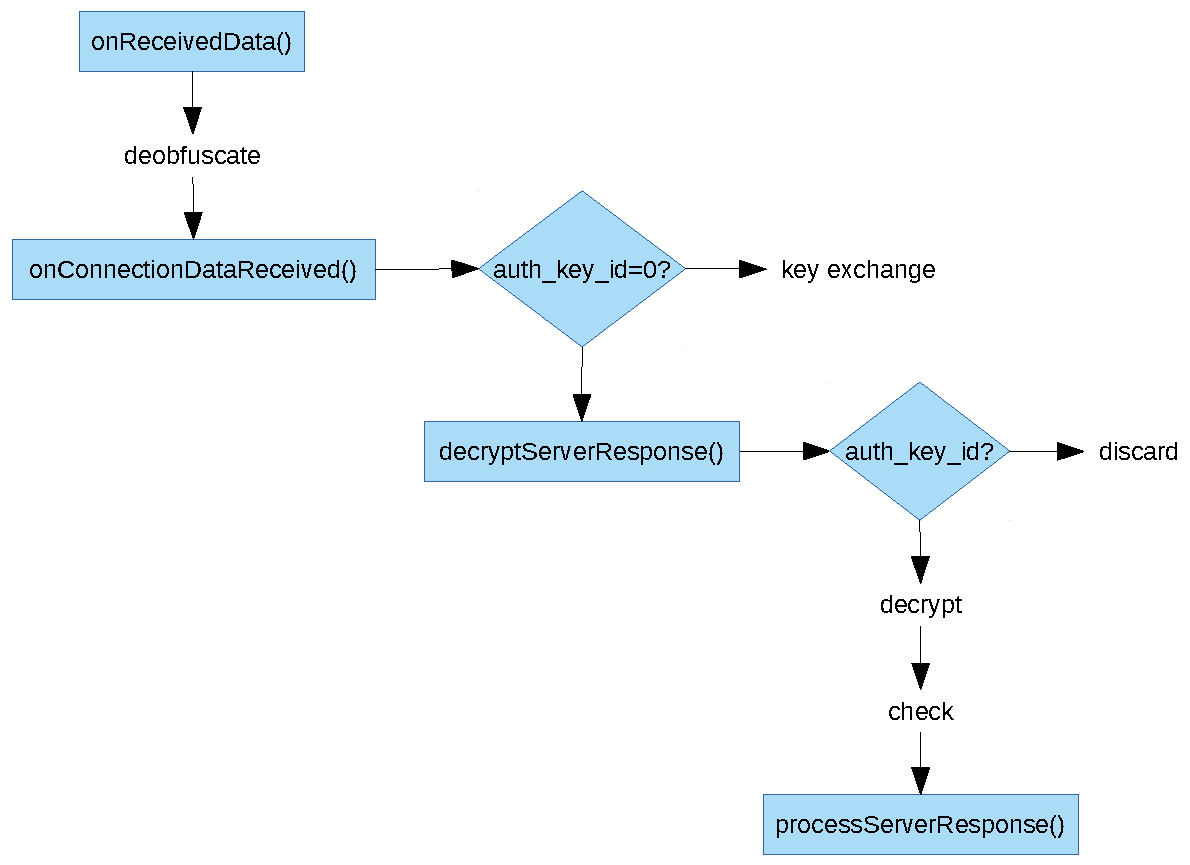
\includegraphics[width=0.99\textwidth]{incoming-flow.pdf}
	\caption[Incoming data processing]{The incoming data are first deobfuscated. If the non-zero \texttt{auth\_key\_id} is valid the message is decrypted and checked if valid. The process is completed by the \texttt{processServerResponse()} function.}
	\label{img:analysis-replay-incoming}
\end{figure}


\subsection{Vulnerability}

A replay attack is an attack where an attacker sniffs sent data by the application and then maliciously resends them another time. Doing so the attacker can repeat any message without the users noticing, of course without actually knowing the message. Protection might be realized by implementing a message counter keeping track of the order messages appear in.

We analyzed how Telegram deals with this issue, see Listing \ref{lst:analysis-replay-check}. Upon the decryption it checks if the message was already processed. The function \texttt{ConnectionSession} holds an internal array of already processed messages. If the message is accepted and processed the message ID is then added into the array.

\begin{listing}[htb]
\caption{Each incoming message is checked whether it was already processed. If not the message is further processed and finally marked as such.
\protect\\ Telegram for Android source code, file \texttt{ConnectionsManager.cpp}, line 728.}
\label{lst:analysis-replay-check}
\begin{minted}{C++}
if (connection->isMessageIdProcessed(messageId)) {
    doNotProcess = true;
}

if (!doNotProcess) {
    // process
    addProcessedMessageId(messageId);
}
\end{minted}
\end{listing}


The behavior we believe might be exploitable is the \texttt{addProcessedMessageId()} function. The function checks the size of the array and if it exceeds 300 it erases the first 100 messages as seen in Listing \ref{lst:analysis-replay-add-processed}.


\begin{listing}[htb]
\caption{After message is successfully processed its ID is added to an internal array of processed messages.
\protect\\ Telegram for Android source code, file \texttt{ConnectionSession.cpp}, line 55.}
\label{lst:analysis-replay-add-processed}
\begin{minted}{C++}
void addProcessedMessageId(messageId)
{
    if (processedMessageIds.size() > 300) {
        processedMessageIds.erase(processedMessageIds.begin(),
            processedMessageIds.begin() + 100);
    }
    processedMessageIds.push_back(messageId);
}
\end{minted}
\end{listing}

The attack scenario is drafted as follows:

\begin{enumerate}
	\item Sniff a message
	\item Wait for 300 other messages
	\item Replace the next message with the first one
	\item Telegram processes the first message again
\end{enumerate}

If Telegram does not provide any additional checks and actually deletes the first 100 IDs the message would be accepted twice. With the attack scenario drafted it is desired to perform the attack.

\subsection{Exploit attempt}

To perform the attack it was first decided to inject a new TCP packet containing the payload copied from the very first packet. That proved to be rather difficult since it's not possible to inject a TCP packet without interfering with the TCP connection. We finally opted for replacing the payload of the next message (i.e. 301st) meaning we would drop its payload and replace it with the first one. That should result in the victim receiving the first message again instead of the new one.

\subsubsection{Required tools}

As found out nor Scapy nor Wireshark are the right tools. Both are useful for passive sniffing and Scapy is capable of sending additional packets but does not allow modification of the packets in real time as it does not reside in the middle of the traffic as described in the Setup, Section \ref{analysis-setup}.

Further, since Telegram uses its own Application layer protocol we were unable to use popular tools such as Fiddler, Burp Suite or OWASP ZAP which are built for HTTP~\cite{fiddler-homepage, burp-homepage}.

Next, the already mentioned Ettercap used to perform the MiM provides simple filtering interface allowing to modify the data routed through. We tried this approach but Ettercap requires the filters to be written in its own language which is very limiting and unfortunately insufficient for our needs.

The scenario was finally tested with Trudy software which can modify any TCP traffic. As its documentation states Trudy is \emph{``a transparent proxy that can modify and drop traffic for arbitrary TCP connections''}~\cite{github-trudy}. All traffic is routed through Trudy which then applies so called \emph{modules}. Trudy modules are bulks of preprogrammed code to perform modifications desired by the user. Trudy provides an example stub of such module and users are encouraged to implement it. Since Trudy is written in Go all modules are to be written in Go as well. To route the traffic and setup the environment properly a prepared virtual machine is available~\cite{github-trudy-vm}.

Upon setting up the MiM as described in \ref{analysis-setup} a virtual machine is run on the computer using Vagrant\footnote{Vagrant is a simple wrapper around a virtualization provider for building complete independent virtual environments.}. The VM installs all required software and Trudy as well. Then it routes all the traffic into and out of Trudy using \texttt{iptables}. Trudy receives all the traffic, modifies it based on the used module and shifts it back to internet as seen in Figure \ref{img:analysis-trudy-setup}.

\begin{figure}[htb]
	\centering
	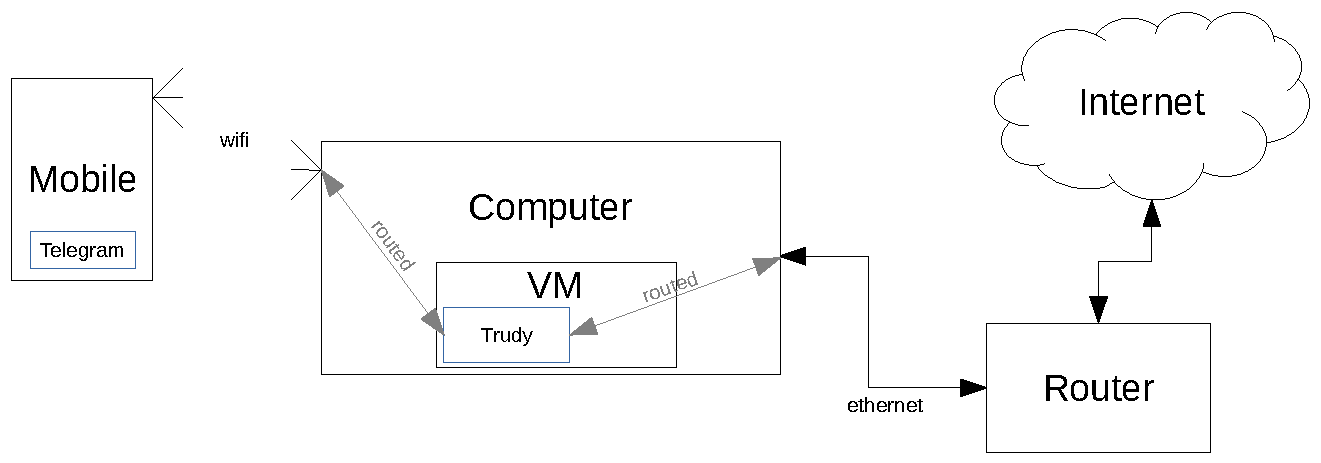
\includegraphics[width=1\textwidth]{setup-trudy.pdf}
	\caption[Trudy setup]{The computer runs Trudy inside a virtual machine. All traffic is routed bidirectionally through Trudy.}
	\label{img:analysis-trudy-setup}
\end{figure}


The implementation of a module for Trudy is straightforward. Trudy calls specific methods in fixed order each designed for one particular action. The methods of a single module are depicted in \ref{img:analysis-trudy-flow} and a description of the methods follows.

\begin{wrapfigure}{r}{0.45\textwidth}
	\centering
	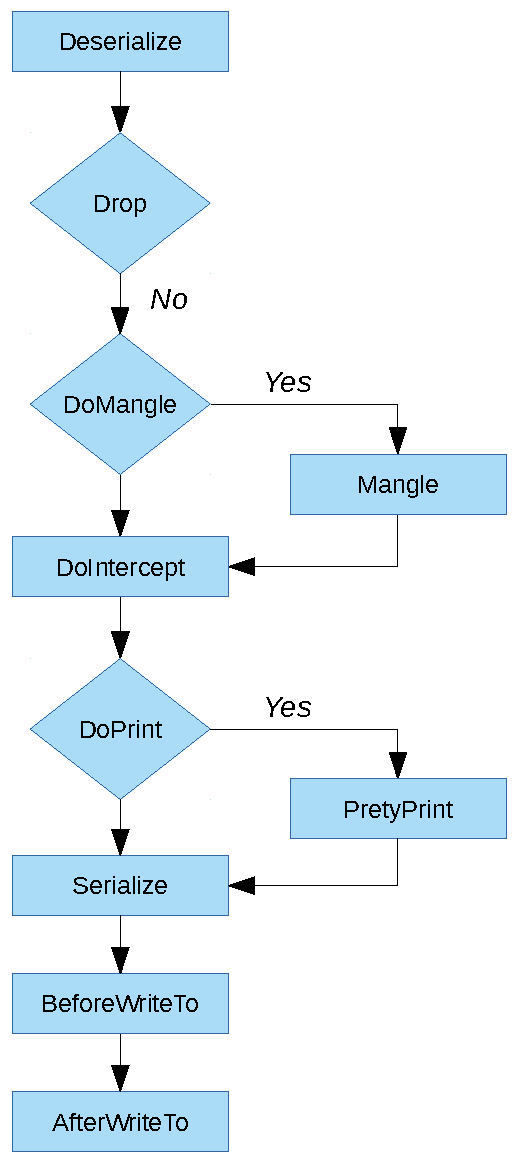
\includegraphics[width=0.34\textwidth]{trudy-flow.pdf}
	\caption[Trudy's data flow]{Trudy module's functions are called in a predefined fixed order.}
	\label{img:analysis-trudy-flow}
\end{wrapfigure}

\begin{itemize}
	\item \textbf{Deserialize()} converts the raw payload into a known structure of data (e.g. HTTP)
	\item \textbf{Drop()} if returns \emph{true} the whole packet is discarded
	\item \textbf{DoMangle()} if returns \emph{true} \texttt{Mangle()} is called
	\item \textbf{Mangle()} alters the payload
	\item \textbf{DoIntercept()} if returns \emph{true} data are sent to the Trudy interceptor\footnote{Trudy interceptor is a simple local website the user may use to interfere with the data. Was not investigated further.}
	\item \textbf{DoPrint()} if returns \emph{true} \texttt{PrettyPrint()} is called
	\item \textbf{PrettyPrint()} prints data in human friendly format
	\item \textbf{Serialize()} converts back to the raw payload if previously deserialized
	\item \textbf{BeforeWriteTo()} actions taken before the data are written to one side or the other
	\item \textbf{AfterWriteTo()} actions taken after the data are written to one side or the other

\end{itemize}


\subsubsection{Preliminaries}

To test our settings we didn't wait for the next 300 messages, rather set up breakpoints on the very lines where Telegram checks if the ID was already processed or not, the line 729 and 859 in the \texttt{ConnectionsManager} file in particular. If the packet was actually send again these breakpoints would be fired and the message further rejected by Telegram. This would confirm our surmise and later improved to comply fully with the scenario.

To further simplify the process we limited all the test messages to the length of 201 bytes to easily identify a message from the other traffic. The length of the message remained the same throughout the testing, we only changed some of the characters each time to see which messages arrived. The testing message we used reads:

\begin{displayquote}
To simplify the process we are using a message longer than 200 bytes to easily identify it in the stream of data
\end{displayquote}

When sending such message through Telegram its length is always equal to 201 bytes under regular conditions.

\subsubsection{Execution}

We've implemented the Trudy module as shown in Listing \ref{lst:analysis-replay-module}. The \texttt{DoMangle()} function checks if the source IP address is equal to one of the Telegram datacenters (\texttt{149.154.167.91:80}). We confirmed our testing application is communicating with this server using Wireshark and as well the configuration details extracted from the \texttt{tgnet.dat} file (see Section \ref{analysis-storage-scripts}) contained a datacenter with such IP address. Further the size of the packet is checked to select the testing messages only.

If those conditions are met the \texttt{Mangle()} function checks whether some bytes were already saved. If not it signifies this is the first message and it copies the TCP payload into the \texttt{oldBytes} array and sets the \texttt{saved} flag to \emph{true}. It does not modify the payload in any way. If \texttt{saved} is already set to \emph{true} it copies the saved bytes into the currently intercepted TCP packet replacing its content. Keep in mind we are attempting the simplified scenario and therefore not waiting for 300 other messages, we are trying to resend the message as soon as another comes which should fire the breakpoints.

\begin{listing}[htb]
\caption{Programmed Trudy module code used to perform a Replay attack on Telegram. The \texttt{DoMangle()} function limits the packet modifications only to our messages. \texttt{Mangle()} actually performs the attack.}
\label{lst:analysis-replay-module}
\begin{minted}{Go}
var saved bool
var oldBytes []byte

func (input Data) DoMangle() bool {
	if input.ServerAddr.String() == "149.154.167.91:80"
		&& len(input.Bytes) == 201 {
		return true
	}
	return false
}

func (input *Data) Mangle() {
	if saved {
		copy(input.Bytes, oldBytes)
	} else {
		oldBytes = make([]byte, len(input.Bytes))
		copy(oldBytes, input.Bytes)
		saved = true
	}
}
\end{minted}
\end{listing}


\subsubsection{Results and Future Work}

Unfortunately it was not the case. We confirmed Telegram successfully  receives the repeated traffic but neither of the desired breakpoints were fired. Further analysis showed Telegram incorrectly deobfuscated the traffic. This is due to the fact that during the communication the \texttt{obf\_enc\_key\_bytes} change periodically. The deobfuscated data are therefore completely different and are rejected on different places as nonsense.

We were unable to continue the attack due to time limitations and the scope of this work. However, we still believe this attack is feasible. In order to continue the obfuscation keys would have to be saved as well. The modified scenario goes as follow:

\begin{enumerate}
	\item Sniff a message, deobfuscate it and save
	\item Wait for 300 other messages
	\item Save the current obfuscation key
	\item Replace the next message with the first one obfuscated by the current key
	\item Telegram processes the first message again
\end{enumerate}

This requires to have the obfuscation capabilities introduced in the C program in Section \ref{analysis-obf-program}. Since Go has a native support of C the codebase could be incorporated into the Trudy module.


\subsubsection{Responsible Disclosure}

The findings were reported to Telegram security team on 7 December 2016 with a kind request for comments. In particular, two points were discussed, the obfuscation method and the Replay attack scenario. The first response from Telegram was received on 12 December 2016.

The obfuscation method was commented only briefly as \emph{``unrelated to data security and is used to counter some of the less sophisticated attempts at banning our service in certain countries''}. In October 2015 Pavel Durov (the founder of Telegram) stated on its Twitter account that Telegram was blocked temporarily in Iran as a result of denied collaboration with the Iranian government~\cite{telegram-durov-iran}. This most likely concerns other countries applying some form of internet censorship but illustrates well that Telegram indeed faces censorship issues.

MTProto has a fixed structure where the \texttt{auth\_key\_id} value is always present at the beginning of the packet and therefore easily recognizable which may be considered as a design flaw of the protocol itself. Another solution to this might be wrapping the protocol into SSL/TLS. The traffic would be then unrecognizable from other protocols based on SSL/TLS such as the very common HTTPS making it even harder to identify. Telegram developers dismissed this proposal considering SSL/TLS as too performance heavy.

Under these circumstances it is understandable why the obfuscation method is not officially documented in any form.

Secondly, Telegram responded to our attack scenario from Section \ref{analysis-attacks} and actually accepted some of our claims. According to the Telegram team the Android application (as opposed allegedly to the other clients such as Telegram for iOS, Telegram Desktop etc.) does not perform one of the the security checks as is required by the protocol, defined in the Security Guidelines for Client Developers in particular \cite{telegram-security-guideline}.

Among other checks, the Security Guideline requires \cite{telegram-security-guideline} the message ID to be checked against the stored ones and Telegram performs that. However, it requires one more additional check -- if the incoming message has lower or equal ID than all the stored IDs such message is to be discarded. This action does indeed mitigate the risk, but Telegram for Android did not carry out this check.
 
The Telegram team further elaborated that this vulnerability does not allow the attacker to cause any severe damage because of the additional protection on the side of the Telegram API. Message actions (sending, editing, deleting, and changing read status), group membership, secret chats, and other important areas are not be affected\footnote{According to Telegram this is due to the checks done in the \texttt{MessagesController.java} class on lines 5731, 5561, 5765, 5817 and other.}. Nevertheless, the Telegram team confirmed the attack would work for nonessential service updates like online or typing statuses. For example, the scenario allowed the attacker to alter the statuses of victim's friends (as seen in the Android application, not in the Telegram network) or spoofing the victim to see typing statuses from contacts not performing such action in reality.

We briefly reviewed theses claims and concluded that the Java part of Telegram application indeed does deal with additional identifiers, such as \texttt{qts}, \texttt{pts} and other. These values do seem to provide additional protection. It is important to note that we did not perform a deeper kind of research.

Telegram promised this will be fixed in the next Android update and offered a financial reward for our findings.




\begin{conclusion}

In the scope of this thesis our objective was to describe a selection of currently used Instant Messenger solutions and discuss its security aspects. Furthermore, to investigate the Telegram Instant Messenger in more detail, mainly its homebrew protocol MTProto and its code.

We have analyzed many security-related incidents and presented their impact on the end user. We have noted how the messengers respond to such incidents, and if they try to improve their security. A number of security related problems still remain. Many messengers are closed-source thus not providing an opportunity for an independent code review, and insufficient or completely missing documentation raises severe questions as well.

Moreover, we have studied the Telegram IM and its MTProto protocol. We have thoroughly documented the protocol's internal working, its initialization and the encryption process. Since Telegram has two types of chat environment (regular and secret chats) we have covered both, and stressed out how they relate to each other. We have noted the cryptographic primitives it uses as well.

We have setup a testing laboratory using various tools, and analyzed the network traffic Telegram produces. We have scrutinized the code base of the official application for Android, and concluded the state of the application is at serious odds with the documentation. This concerns mainly the undocumented obfuscation method Telegram uses. The MTProto traffic is encrypted one more time with the key and IV appended in front of the data. This has no effect on the data security, and is easily debunked by the deobfuscation program we have implemented. When the Telegram team was confronted with these claims, they noted the method is used to defy some of the less sophisticated methods of censorship in certain countries.

Finally, we have localized an exploitable vulnerability and drafted an attack scenario. We concluded the Android application does not check message identification numbers properly and that a Replay attack might be feasible. Although our primary scenario of the attack turned out not to be applicable, we have drafted a new altered scenario which we believe could be. We have reported our findings to the Telegram security team which accepted our remarks and agreed, to a certain degree, this might be exploitable. Telegram promised to fix this issue in the next software release.

Our work mainly focused on the protocol and the Android client, but there are still many areas where further research might be required. Other research might focus on the other Telegram clients, such as the desktop or iOS version, studying the protocol as a whole or applying other forms of attacks.


\end{conclusion}


\bibliographystyle{iso690}
\bibliography{ref}

\appendix

% \printglossaries

\chapter{Contents of CD}\label{app:CDcontent}

Visualise the contents of enclosed media. Use of \verb|dirtree| is recommended. Note that directories src and text with appropriate contents are mandatory.


\begin{figure}
	\dirtree{%
		.1 readme.txt\DTcomment{the file with CD contents description}.
		.1 data\DTcomment{the data files directory}.
		.2 graphs\DTcomment{the directory of graphs of experiments}.
		.3 *.eps\DTcomment{the B/W graphs}.
		.3 *.png\DTcomment{the color g<raphs}.
		.3 *.dat\DTcomment{the graphs data files}.
		.1 exe\DTcomment{the directory with executable WBDCM program}.
		.2 wbdcm\DTcomment{the WBDCM program executable (UNIX)}.
		.2 wbdcm.exe\DTcomment{the WBDCM program executable (Windows)}.
		.1 src\DTcomment{the directory of source codes}.
		.2 wbdcm\DTcomment{the directory of WBDCM program}.
		.3 Makefile\DTcomment{the makefile of WBDCM program (UNIX)}.
		.2 thesis\DTcomment{the directory of \LaTeX{} source codes of the thesis}.
		.3 figures\DTcomment{the thesis figures directory}.
		.3 *.tex\DTcomment{the \LaTeX{} source code files of the thesis}.
		.1 text\DTcomment{the thesis text directory}.
		.2 thesis.pdf\DTcomment{the Diploma thesis in PDF format}.
		.2 thesis.ps\DTcomment{the Diploma thesis in PS format}.
	}
\end{figure}


\end{document}
